\documentclass[english]{mrl}

\usepackage{float}
\usepackage[utf8]{inputenc}
\usepackage[english]{babel}

\theoremstyle{plain}
\newtheorem{prop}{\protect\propositionname}

\usepackage{amsmath}
\usepackage{amssymb}
\usepackage{amsfonts}
\usepackage{bm}
\usepackage[stable,splitrule]{footmisc}
\usepackage[usenames,dvipsnames]{xcolor}
\usepackage{setspace}
\AtBeginDocument{\let~=\nobreakspace}

\usepackage{lineno}
\linenumbers

\usepackage{draftwatermark}
\SetWatermarkText{DRAFT}
\SetWatermarkScale{7}
\SetWatermarkLightness{0.95}

\hypersetup{colorlinks=false}
\usepackage{booktabs}
\usepackage{caption}
\usepackage{longtable}
\usepackage[T1]{fontenc}
\usepackage{geometry}
\geometry{verbose,tmargin=2cm,bmargin=2cm,lmargin=2cm,rmargin=2cm}
\usepackage{array}
\usepackage{url}
\usepackage{multirow}

\hypersetup{
    bookmarks=true,
    unicode=false,
    pdftitle={Autonomous System Deduplication for Monero Node Peer Selection},
    pdfauthor={Jean-Claude Sonnet, Giorgio Pretrani Trasformi, Qwen Stefani},
    pdfsubject={},
    pdfcreator={plowsof},
    pdfproducer={},
    pdfkeywords={},
    colorlinks=false
}

\newcommand{\nReachNew}{3,983}
\newcommand{\nHonestNew}{2,690}
\newcommand{\nSpyNew}{1,293}
\newcommand{\hTwentyFourNew}{1,983}
\newcommand{\hAsnNew}{573}
\newcommand{\hSixteenNew}{1,273}
\newcommand{\spyTwentyFourNew}{1,132}
\newcommand{\spyAsnNew}{10}
\newcommand{\thresholdNew}{3.46}
\newcommand{\pObsTwentyFourNew}{36.2}
\newcommand{\pObsAsnNew}{1.07}
\newcommand{\spyTopAsnNew}{14061}
\newcommand{\spyTopAsnNNew}{1,279}
\newcommand{\spyTopAsnPctNew}{98.9}
\newcommand{\honestInSpyTopAsnNew}{630}
\newcommand{\pSSNew}{39.5}
\newcommand{\pAAequalNew}{69.3}
\newcommand{\pASNew}{1.72}
\newcommand{\kStarNew}{374}
\newcommand{\nReachOld}{4,607}
\newcommand{\nHonestOld}{2,764}
\newcommand{\nSpyOld}{1,843}
\newcommand{\hTwentyFourOld}{2,647}
\newcommand{\hAsnOld}{794}
\newcommand{\hSixteenOld}{1,903}
\newcommand{\spyTwentyFourOld}{257}
\newcommand{\spyAsnOld}{7}
\newcommand{\thresholdOld}{3.33}
\newcommand{\pObsTwentyFourOld}{8.8}
\newcommand{\pObsAsnOld}{0.73}
\newcommand{\spyTopAsnOld}{54098}
\newcommand{\spyTopAsnNOld}{566}
\newcommand{\spyTopAsnPctOld}{30.7}
\newcommand{\honestInSpyTopAsnOld}{0}
\newcommand{\pSSOld}{41.0}
\newcommand{\pAAequalOld}{69.9}
\newcommand{\pASOld}{0.87}
\newcommand{\kStarOld}{553}
\newcommand{\simOldAsmapEightyMean}{0.09}
\newcommand{\simOldAsmapEightyPct}{0.7}
\newcommand{\simOldAsmapEightyInMedian}{37}
\newcommand{\simOldAsmapEightyInMax}{372}
\newcommand{\simOldAsmapNinetyMean}{0.09}
\newcommand{\simOldAsmapNinetyPct}{0.7}
\newcommand{\simOldAsmapNinetyInMedian}{78}
\newcommand{\simOldAsmapNinetyInMax}{738}
\newcommand{\simOldHybridEightyMean}{0.56}
\newcommand{\simOldHybridEightyPct}{4.7}
\newcommand{\simOldHybridEightyInMedian}{96}
\newcommand{\simOldHybridEightyInMax}{140}
\newcommand{\simOldHybridNinetyMean}{0.56}
\newcommand{\simOldHybridNinetyPct}{4.7}
\newcommand{\simOldHybridNinetyInMedian}{204}
\newcommand{\simOldHybridNinetyInMax}{272}
\newcommand{\simOldSubnetEightyMean}{1.06}
\newcommand{\simOldSubnetEightyPct}{8.8}
\newcommand{\simOldSubnetEightyInMedian}{87}
\newcommand{\simOldSubnetEightyInMax}{121}
\newcommand{\simOldSubnetNinetyMean}{1.05}
\newcommand{\simOldSubnetNinetyPct}{8.8}
\newcommand{\simOldSubnetNinetyInMedian}{182}
\newcommand{\simOldSubnetNinetyInMax}{227}
\newcommand{\simNewAsmapEightyMean}{0.13}
\newcommand{\simNewAsmapEightyPct}{1.1}
\newcommand{\simNewAsmapEightyInMedian}{7}
\newcommand{\simNewAsmapEightyInMax}{452}
\newcommand{\simNewAsmapNinetyMean}{0.13}
\newcommand{\simNewAsmapNinetyPct}{1.1}
\newcommand{\simNewAsmapNinetyInMedian}{14}
\newcommand{\simNewAsmapNinetyInMax}{877}
\newcommand{\simNewHybridEightyMean}{0.78}
\newcommand{\simNewHybridEightyPct}{6.5}
\newcommand{\simNewHybridEightyInMedian}{81}
\newcommand{\simNewHybridEightyInMax}{190}
\newcommand{\simNewHybridNinetyMean}{0.78}
\newcommand{\simNewHybridNinetyPct}{6.5}
\newcommand{\simNewHybridNinetyInMedian}{165}
\newcommand{\simNewHybridNinetyInMax}{362}
\newcommand{\simNewSubnetEightyMean}{4.35}
\newcommand{\simNewSubnetEightyPct}{36.3}
\newcommand{\simNewSubnetEightyInMedian}{67}
\newcommand{\simNewSubnetEightyInMax}{110}
\newcommand{\simNewSubnetNinetyMean}{4.35}
\newcommand{\simNewSubnetNinetyPct}{36.3}
\newcommand{\simNewSubnetNinetyInMedian}{142}
\newcommand{\simNewSubnetNinetyInMax}{198}
\newcommand{\ctrlHosts}{157}
\newcommand{\ctrlIps}{145}
\newcommand{\ctrlInData}{80}
\newcommand{\ctrlFlagged}{0}
\newcommand{\nPriceAsns}{9}
\newcommand{\nPriceProviders}{9}
\newcommand{\priceMin}{3.00}
\newcommand{\priceMax}{6.72}
\newcommand{\priceMaxRatio}{1.68}
\newcommand{\nDcList}{933}
\newcommand{\nHonestDcAsn}{99}
\newcommand{\nHonestDcNodes}{1,633}
\newcommand{\nHonestNonDcAsn}{474}
\newcommand{\supSubnetKIX}{4.71}
\newcommand{\supAsmapKIX}{0.15}
\newcommand{\supHybridKIX}{3.79}
\newcommand{\supSubnetKXCIX}{4.71}
\newcommand{\supAsmapKXCIX}{1.61}
\newcommand{\supHybridKXCIX}{5.23}
\newcommand{\supSubnetKCMXXXIII}{4.71}
\newcommand{\supAsmapKCMXXXIII}{7.49}
\newcommand{\supHybridKCMXXXIII}{5.30}
\newcommand{\supSubnetKCC}{4.71}
\newcommand{\supAsmapKCC}{3.03}
\newcommand{\supHybridKCC}{5.31}
\newcommand{\supSubnetKCCC}{4.71}
\newcommand{\supAsmapKCCC}{4.09}
\newcommand{\supHybridKCCC}{5.32}
\newcommand{\supSubnetKCD}{4.71}
\newcommand{\supAsmapKCD}{4.98}
\newcommand{\supHybridKCD}{5.33}
\newcommand{\supSubnetKDC}{4.71}
\newcommand{\supAsmapKDC}{6.21}
\newcommand{\supHybridKDC}{5.32}
\newcommand{\kBreakEven}{370}
\newcommand{\respAsmapROneNew}{8.31}
\newcommand{\respSubnetObsNew}{4.38}
\newcommand{\respSubnetROneNew}{4.71}
\newcommand{\respAsmapROneOld}{8.37}
\newcommand{\respSubnetObsOld}{1.05}
\newcommand{\respSubnetROneOld}{4.92}
\newcommand{\inAloneSubnet}{151}
\newcommand{\inAloneMaxSubnet}{192}
\newcommand{\inBigSubnet}{87}
\newcommand{\nAloneSubnet}{357}
\newcommand{\inAloneAsmap}{801}
\newcommand{\inAloneMaxAsmap}{877}
\newcommand{\inBigAsmap}{3}
\newcommand{\nAloneAsmap}{357}
\newcommand{\inAloneHybrid}{302}
\newcommand{\inAloneMaxHybrid}{362}
\newcommand{\inBigHybrid}{26}
\newcommand{\nAloneHybrid}{357}
\newcommand{\torAses}{977}
\newcommand{\torDc}{173}
\newcommand{\btcAses}{1,230}
\newcommand{\btcDc}{132}
\newcommand{\unionAses}{1,978}
\newcommand{\unionDc}{233}
\newcommand{\unionDcTwo}{117}
\newcommand{\unionUnlisted}{1,745}
\newcommand{\crawlIps}{98,483}
\newcommand{\crawlAsns}{4,953}
\newcommand{\crawlAsnsDc}{274}
\newcommand{\crawlReachIps}{4,018}
\newcommand{\crawlReachAsns}{604}
\newcommand{\crawlStart}{2026-09-28}
\newcommand{\bitnodesTime}{2026-10-05 20:24}
\newcommand{\banAddresses}{4,001}
\newcommand{\banAsns}{9}
\newcommand{\pegIps}{1,925}
\newcommand{\pegAsns}{3}
\newcommand{\svn}{100}
\newcommand{\svFrame}{1,978}
\newcommand{\svR}{24}
\newcommand{\svU}{29}
\newcommand{\svN}{47}
\newcommand{\svPriced}{10}
\newcommand{\svCheap}{8}
\newcommand{\svCheapV}{5}
\newcommand{\svTaggedinSample}{20}
\newcommand{\svUntaggedR}{4}
\newcommand{\svVpshTotal}{2,257}
\newcommand{\svKR}{475}
\newcommand{\svKRLoLo}{330}
\newcommand{\svKRHiHi}{657}
\newcommand{\svKRU}{1,048}
\newcommand{\svKRULoLo}{856}
\newcommand{\svKRUHiHi}{1,236}
\newcommand{\svKCheap}{158}
\newcommand{\svKCheapLoLo}{81}
\newcommand{\svKCheapHiHi}{297}
\newcommand{\svKCheapV}{99}
\newcommand{\svKCheapVLoLo}{43}
\newcommand{\svKCheapVHiHi}{221}
\newcommand{\svTagRecall}{0.83}
\newcommand{\svKGlobalHosting}{2,719}
\newcommand{\banProbed}{2,440}
\newcommand{\banReach}{2,025}
\newcommand{\banReachPct}{83.0}
\newcommand{\banTwentyFour}{68}
\newcommand{\banAsnsReach}{3}
\newcommand{\banTopAsn}{401476}
\newcommand{\banTopAsnN}{1,965}
\newcommand{\stemObsCur}{36.5}
\newcommand{\stemObsDiv}{12.3}
\newcommand{\stemObsAnyCur}{59.7}
\newcommand{\stemObsAnyDiv}{24.3}
\newcommand{\stemWorstCur}{39.2}
\newcommand{\stemWorstDiv}{42.5}
\newcommand{\stemWorstAsmap}{69.3}
\newcommand{\stemBanCur}{37.5}
\newcommand{\stemBanDiv}{13.9}
\newcommand{\stemOldCur}{8.8}
\newcommand{\stemOldDiv}{6.2}
\newcommand{\banOutSubnet}{4.51}
\newcommand{\banOutAsmap}{0.15}
\newcommand{\beMean}{377}
\newcommand{\beSd}{5}
\newcommand{\beMin}{369}
\newcommand{\beMax}{382}
\newcommand{\beSeeds}{6}
\newcommand{\beRatioMid}{383}
\newcommand{\beRatioHigh}{398}
\newcommand{\stemObsOut}{4.38}
\newcommand{\plNodes}{2,527}
\newcommand{\plListSpy}{17.5}
\newcommand{\plUnknown}{28.5}
\newcommand{\plSubnetObs}{2.73}
\newcommand{\plAsmapObs}{0.71}
\newcommand{\plCapThreeObs}{0.66}
\newcommand{\plCapOneObs}{0.26}
\newcommand{\plSubnetSpr}{2.73}
\newcommand{\plAsmapSpr}{3.35}
\newcommand{\plCapThreeSpr}{3.21}
\newcommand{\plCapOneSpr}{3.59}
\newcommand{\plStemCurObs}{22.7}
\newcommand{\plStemDivObs}{10.7}
\newcommand{\plStemCurSpr}{22.7}
\newcommand{\plStemDivSpr}{25.0}
\newcommand{\plBanSubnetObs}{2.42}
\newcommand{\plSubnetObsPct}{22.7}
\newcommand{\loadMedCur}{0.75}
\newcommand{\loadMedDiv}{1.03}
\newcommand{\loadMaxCur}{1.83}
\newcommand{\loadMaxDiv}{3.10}
\newcommand{\loadGiniCur}{0.29}
\newcommand{\loadGiniDiv}{0.40}
\newcommand{\loadAloneCur}{0.86}
\newcommand{\loadAloneDiv}{1.45}
\newcommand{\stemTopTenDiv}{36.7}
\newcommand{\stemTopThirtyDiv}{40.4}
\newcommand{\stemMimicDiv}{38.0}
\newcommand{\abHours}{8.9}
\newcommand{\abInst}{12}
\newcommand{\abBoxes}{4}
\newcommand{\abCtrlPct}{33.8}
\newcommand{\abAsmapPct}{2.7}
\newcommand{\abCtrlTwelve}{4.05}
\newcommand{\abAsmapTwelve}{0.32}
\newcommand{\abCtrlAsns}{7.0}
\newcommand{\abAsmapAsns}{12.0}
\newcommand{\abCtrlStemDiv}{13.8}
\newcommand{\abCtrlMin}{17}
\newcommand{\abCtrlMax}{58}
\newcommand{\abAsmapMax}{8}
\newcommand{\stemNineNineDiv}{41.9}
\newcommand{\stemNineNineAsmap}{13.4}
\newcommand{\stemThreeSeventyAsmap}{39.7}
\newcommand{\stemObsAlpha}{22.8}
\newcommand{\stemWorstAlpha}{41.1}
\newcommand{\stemRegretDiv}{3.3}
\newcommand{\stemRegretAlpha}{1.9}
\newcommand{\abPeersMin}{12}
\newcommand{\abPeersMax}{18}
\newcommand{\abRankP}{3.7\times10^{-7}}
\newcommand{\abAsmapMin}{0}
\newcommand{\stemObsGain}{24.2}
\newcommand{\fpDoN}{1,279}
\newcommand{\fpDoPids}{1,279}
\newcommand{\fpDoTip}{99.7}
\newcommand{\fpHonTip}{97.1}
\newcommand{\fpDoUnpruned}{99.8}
\newcommand{\fpHonUnpruned}{67.0}
\newcommand{\fpDoRpc}{99.7}
\newcommand{\fpHonRpc}{59.4}
\newcommand{\fpDoPort}{100}
\newcommand{\spyShareOfTopAsn}{67}
\newcommand{\spySixteenNew}{77}
\newcommand{\ishAloneNodes}{13}
\newcommand{\ishAloneMaster}{18}
\newcommand{\ishAloneAsmap}{62}
\newcommand{\ishBigNodes}{63}
\newcommand{\ishBigMaster}{51}
\newcommand{\ishBigAsmap}{4}
\newcommand{\banAdoptPct}{72}
\newcommand{\banAdoptOthersPct}{14}
\newcommand{\ikMoreNodes}{764}
\newcommand{\ikMorePct}{28}
\newcommand{\ikMoreMaxK}{4}
\newcommand{\ikSingleAsesPct}{62}
\newcommand{\ikTwoAsmap}{402}
\newcommand{\ikThreeAsmap}{267}
\newcommand{\ikFourAsmap}{200}
\newcommand{\lpAloneDefault}{11}
\newcommand{\lpAloneAsmap}{46}
\newcommand{\lpBigDefault}{53}
\newcommand{\lpBigAsmap}{13}
\newcommand{\lpPeersDefault}{92}
\newcommand{\lpPeersAsmap}{132}


\title{Autonomous System Deduplication for Monero Node Peer Selection\\\vspace{.3cm}
\large Draft v0.1}
\authors{Jean-Claude Sonnet, Giorgio Pretrani Trasformi and Qwen Stefani}
\affiliations{Monero Project contributor. Method, simulation code and game-theoretic model adapted from Rucknium (Monero Research Lab)}
\date{\today}

\type{RESEARCH NOTE}
\ident{DRAFT}

\makeatother

\providecommand{\propositionname}{Proposition}

\begin{document}

\begin{abstract}
Monero nodes deduplicate outbound peer candidates by /24 subnet (pull request \#9939), following Rucknium \cite{Rucknium2025}. Pull request \#11474 adds an opt-in \texttt{--asmap} option that deduplicates by autonomous system (AS) instead. This note applies Rucknium's simulation and game to AS deduplication. In October 2026 the suspected spy nodes occupy \spyTwentyFourNew{} /24 subnets, but \spyTopAsnPctNew{} percent of them are in one AS. Against them, AS deduplication reduces an honest node's outbound connections to suspected spy nodes from \simNewSubnetEightyMean{} to \simNewAsmapEightyMean{} out of 12 in simulation, and from \abCtrlPct{} to \abAsmapPct{} percent on live nodes. Honest nodes, however, occupy \thresholdNew{} times more /24 subnets than ASes, so an adversary that spreads over many ASes does better against AS deduplication. Servers in other ASes cost about the same as bulk servers, so the number of rentable ASes decides. AS deduplication stays better while the adversary can rent servers in fewer than about \kBreakEven{} ASes, and a sample survey estimates \svKR{} (\svKRLoLo{} to \svKRHiHi) rentable ASes among those that already host Tor, Bitcoin or Monero servers. The results support AS deduplication as an opt-in option, not as the default. Choosing Dandelion++ stems uniformly over the ASes of the outbound connections, without changing peer selection, reduces the probability that a stem is a suspected spy node from \stemObsCur{} to \stemObsDiv{} percent, and costs at most \stemRegretDiv{} percentage points against every adversary placement simulated.
\end{abstract}

\section{Statement of the problem}

Spy nodes can reduce the effectiveness of Dandelion++ \cite{Fanti2018a}. Rucknium showed that an adversary can exploit bulk prices for whole subnets, and that deduplicating outbound peer candidates by /24 subnet reduces the share of an honest node's outbound connections made to suspected spy nodes from 30.8 to 8.8 percent \cite{Rucknium2025}. The deduplication was implemented in Monero pull request \#9939 \cite{MoneroPR9939}.

Subnet deduplication assumes that the adversary's nodes are packed into few subnets. An adversary that rents virtual servers from a large cloud provider gets addresses scattered over many /24 subnets, but all of them inside the provider's autonomous system (AS). An AS is a network under a single routing policy, identified by an AS number (ASN). Bitcoin Core has grouped peers by ASN, using a map from IP prefixes to ASNs called an \emph{asmap}, since 2020 \cite{BitcoinPR16702}. Monero pull request \#11474 \cite{MoneroPR11474}, a revival of \#7935 \cite{MoneroPR7935}, adds an opt-in \texttt{--asmap} option that groups peers by ASN for outbound peer selection.

When this was discussed on 5 October 2026, Rucknium accepted AS grouping as an opt-in option and stated the conditions for making it the default \cite{NWLB20261005}: an analysis showing ``with reasonable confidence, that the cure would not be worse than the disease'', as was done for /24 deduplication. He raised four concerns, which this note addresses in turn:
\begin{enumerate}
\item An adversary could spread across many ASNs in response to a default rollout, making the problem worse.
\item Many honest nodes are concentrated in the ASNs of server providers, so an adversary could exploit AS avoidance to obtain more outbound connections than honest nodes.
\item ASNs are harder to analyze than subnets because ASNs do not have a defined size.
\item Nodes in sparsely populated ASNs would receive many more inbound connections.
\end{enumerate}

\section{Background}

\subsection{Peer selection with /24 and AS deduplication}

The selection rule is implemented in \texttt{make\_new\_connection\_from\_peerlist()} in \texttt{src/p2p/net\_node.inl} \cite{MoneroPR11474}. For each new outbound connection in the public zone, a node:
\begin{enumerate}
\item collects the \emph{groups} of its current connections. Without \texttt{--asmap} the group of an IPv4 address is its /24 subnet. With \texttt{--asmap} the group is the ASN that the asmap returns, and only outbound connections are counted;
\item shuffles its peer list and keeps the first candidate of each group that is not already a connected group;
\item picks one of the remaining candidates.
\end{enumerate}
After steps 1 and 2 there is one candidate per group, so the probability of selecting a group does not depend on how many addresses the group contains. Appendix \ref{sec:appendix-draw} shows that, when the final pick is uniform, the draw is equivalent to choosing a non-connected group uniformly and then a member of that group uniformly. This is why the size of an AS, concern 3 above, does not enter the analysis of an AS that contains only adversary nodes: a large AS and an AS with a single node are each one group.

Bitcoin Core connects out to at most one peer per network group, which is the ASN when an asmap is used, and also uses the group to place addresses in its address manager buckets \cite{BitcoinInit,BitcoinPR16702}; candidates in an already connected group are skipped (\texttt{src/net.cpp}, line 2915, same commit). It does not deduplicate candidates in the way described above. Its asmap was introduced against AS-level routing attacks and eclipse attacks \cite{Apostolaki2017,Tran2020,Heilman2015}, not against spy nodes. It is opt-in in Bitcoin Core: \texttt{-asmap} with no file uses an embedded map and \texttt{-asmap=<file>} reads a map from disk \cite{BitcoinInit,BitcoinPR28792}. Eclipse attacks on Monero's peer-to-peer network are analyzed by \cite{Shi2025}.

\subsection{The asmap}

Pull request \#11474 embeds \texttt{2026/1788801420\_asmap.dat} from the \texttt{bitcoin-core/asmap-data} repository \cite{AsmapData,MoneroPR11474}. It is a ``filled'' map: in this note's own lookup of the map, every one of the $2^{32}$ IPv4 addresses resolves to an ASN, and 82,443 distinct ASNs appear in the IPv4 part of the map (replication code: \texttt{asmap\_coverage.py}). The fallback to /24 groups for unmapped addresses in pull request \#11474 is therefore never used for IPv4, and an adversary cannot use unmapped address space to get one group per /24.

\section{Data}

\noindent{\fboxrule 2pt\fbox{\begin{minipage}[t]{1\columnwidth - 2\fboxsep - 2\fboxrule}%

\subsection{Box: Data and suspected spy node classification\label{sec:box-data}}

\textbf{October 2026 data.} Reachable Monero nodes were collected by a crawler running on four vantage points \cite{Observatory}. A node is \emph{reachable} if a handshake to its advertised address succeeded. The snapshot was taken on 2026-10-05 at 16:19 UTC and contains \nReachNew{} distinct reachable IPv4 addresses.

A node was classified as a suspected spy node if its handshake showed one of two protocol fingerprints that an unmodified \texttt{monerod} does not produce. The fingerprints are withheld from this public draft so that the operators cannot evade them, and are available to the Monero Research Lab on request. As a check for false positives, the classifier was applied to the default remote nodes in the Monero GUI pull request \#4601 \cite{GuiRemoteNodes}: of \ctrlHosts{} hosts, \ctrlIps{} IPv4 addresses resolved, \ctrlInData{} of them were in the reachable dataset, and \ctrlFlagged{} of those were classified as suspected spy nodes.

\textbf{Ban-listed nodes.} The crawler does not handshake addresses in the MRL ban list \cite{MRLBanList}, version 2, so the snapshot contains none of them. To measure them, every ban-listed IPv4 address that peers gossiped to the crawler, \banProbed{} in total, was handshaked from the four vantage points on 2026-10-05 (replication code: \texttt{ban\_crawl.py}). \banReach{} (\banReachPct{} percent) completed a handshake. They occupy \banTwentyFour{} /24 subnets and \banAsnsReach{} ASNs, \banTopAsnN{} of them in AS\banTopAsn{} (SCNL-1-0001 \cite{IPtoASN}). They are added to the October 2026 data in Section \ref{sec:stem} to represent a node that does not use the ban list, which is the default.

\textbf{May 2025 data.} To make the results reproducible without the withheld classification, the network simulations and the price-premium response are repeated on the data used in \cite{Rucknium2025}: the \texttt{good\_peers} network scan and the \texttt{ban\_list\_v1} ban list from the \texttt{xmrpeers} R package \cite{xmrpeers}, cleaned with the same code. This gives \nReachOld{} reachable IPv4 addresses, of which \nSpyOld{} are in the ban list, the same totals as in \cite{Rucknium2025}.

\textbf{ASNs.} All addresses in both datasets are mapped to ASNs with the asmap embedded by pull request \#11474. The May 2025 addresses are therefore mapped with a map from 2026.%
\end{minipage}}}

\bigskip

Table \ref{table-concentration} summarizes how the nodes in each dataset are grouped. In October 2026, the \nSpyNew{} suspected spy nodes occupy \spyTwentyFourNew{} distinct /24 subnets but only \spyAsnNew{} ASNs; \spyTopAsnNNew{} of them (\spyTopAsnPctNew{} percent) are in AS\spyTopAsnNew{}, which also hosts \honestInSpyTopAsnNew{} honest reachable nodes. /24 deduplication leaves almost one group per suspected spy node, while AS deduplication reduces them to a few groups. Honest nodes are less concentrated: \nHonestNew{} honest nodes occupy \hTwentyFourNew{} /24 subnets and \hAsnNew{} ASNs.

\textbf{What the label means.} Both fingerprints show that a node runs modified software. Neither shows what its operator does with the connections it receives, so ``suspected spy node'' is an inference and should be read as ``node of a large fleet running modified software''. AS\spyTopAsnNew{} is DigitalOcean (DIGITALOCEAN-ASN \cite{IPtoASN}). The fleet is \spyShareOfTopAsn{} percent of the reachable Monero nodes in that AS, not a large part of DigitalOcean; the AS that hosts a node is not necessarily its operator. The fleet is uniform. Of its \fpDoN{} nodes in AS\spyTopAsnNew{}, \fpDoPort{} percent listen on the default port, \fpDoTip{} percent are within 10 blocks of the chain tip (honest nodes: \fpHonTip{}), \fpDoUnpruned{} percent are unpruned (honest: \fpHonUnpruned{}) and \fpDoRpc{} percent advertise an RPC port (honest: \fpHonRpc{}), and every node has its own peer ID (replication code: \texttt{fleet\_profile.py}). This is consistent with a single deployment, but the distinct peer IDs mean that a single operator cannot be shown from the handshake. \cite{Kopyciok2026} describe the same pattern, many anomalous peers concentrated in one AS that promotes its own addresses, for June 2025, and argue that a consistent deviation from the network baseline is significant for security ``regardless of ultimate intent''. That AS, LIONLINK-NETWORKS (AS54098), is also the largest AS among the ban-listed nodes in the May 2025 data (\spyTopAsnNOld{} nodes), and it announces the address ranges of the entity that b10c calls LinkingLion in the Bitcoin network \cite{b10c2024}. Benign explanations for the October 2026 fleet, such as a commercial remote-node service or a measurement project, cannot be excluded. None of the results in this note depends on intent: they measure how many of an honest node's outbound connections and Dandelion++ stems one concentrated fleet obtains, which bounds what it could learn whether or not it records transactions \cite{Fanti2018a,Sharma2022}.

\begin{table}[t]
\caption{
{\fontsize{20}{25}\selectfont  Grouping of reachable nodes by /16 subnet, /24 subnet, and autonomous system}
} 
\begin{tabular*}{\linewidth}{@{\extracolsep{\fill}}llrrrrr}
\toprule
Dataset & Nodes & IP addresses & /16 subnets & /24 subnets & ASNs & Effective ASNs \\ 
\midrule\addlinespace[2.5pt]
Oct 2026 & Suspected spy & 1,293 & 77 & 1,132 & 10 & 1.0 \\ 
Oct 2026 & Honest & 2,690 & 1,273 & 1,983 & 573 & 13.2 \\ 
May 2025 & Honest & 2,764 & 1,903 & 2,647 & 794 & 61.9 \\ 
May 2025 & Suspected spy & 1,843 & 61 & 257 & 7 & 5.5 \\ 
\bottomrule
\end{tabular*}
\label{table-concentration}
\end{table}


Figure \ref{fig:treemap-asn} plots every reachable node in October 2026, grouped by ASN (black perimeters) and /24 subnet (yellow perimeters), in the style of \cite{Rucknium2025}. Figure \ref{fig:treemap-dedup} shows the groups that remain after deduplication, coloured by the share of suspected spy nodes in each group.

\begin{figure}[H]
\caption{ASN treemap of honest and suspected spy nodes, October 2026}
\label{fig:treemap-asn}
\centering{}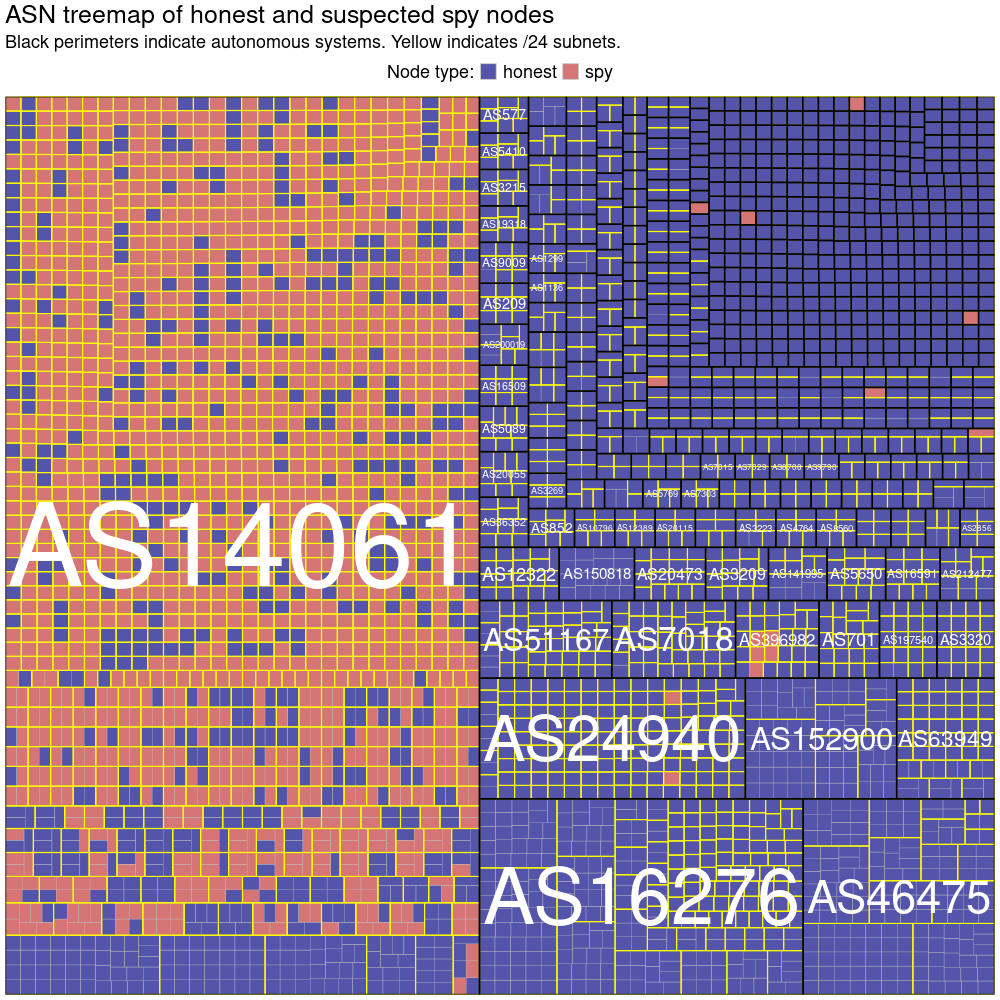
\includegraphics[scale=0.45]{images/treemap-asn}
\end{figure}

\begin{figure}[H]
\caption{Groups after deduplication, October 2026: left, /24 deduplication (monero master); right, AS deduplication (\texttt{--asmap})}
\label{fig:treemap-dedup}
\centering{}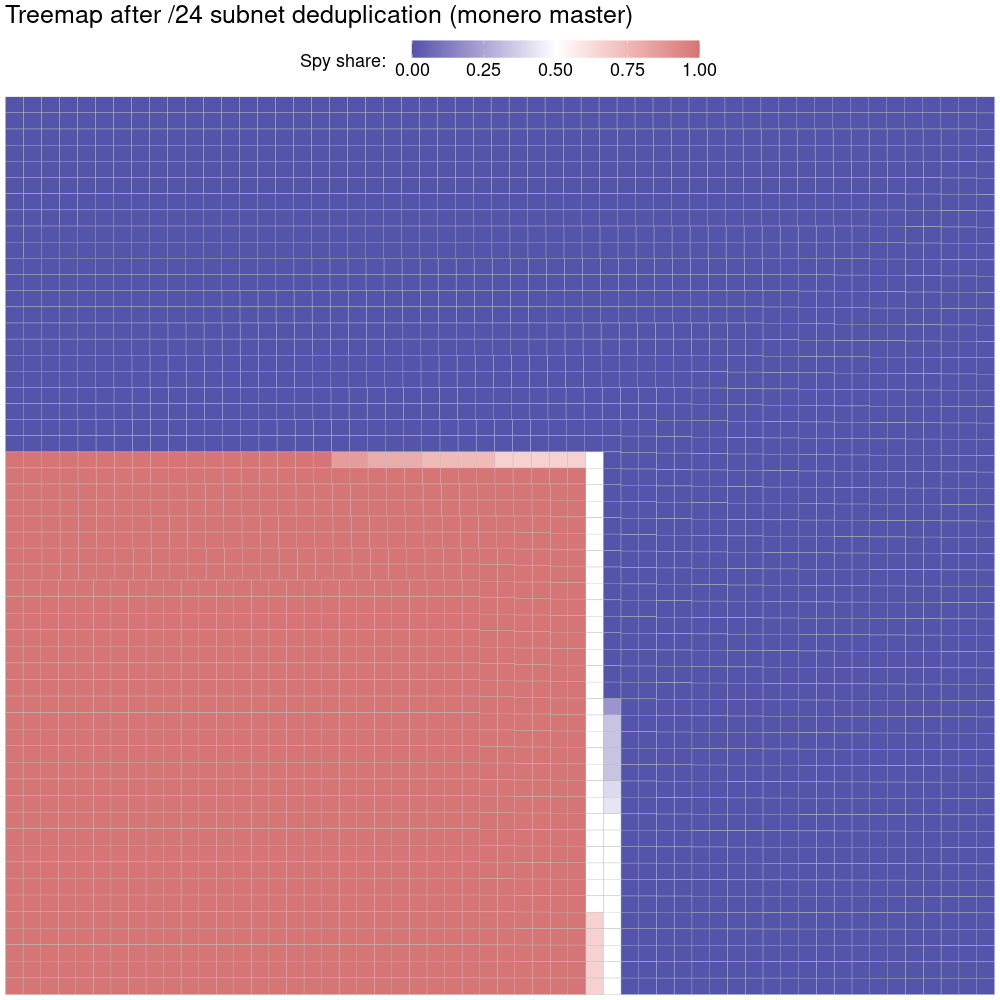
\includegraphics[width=0.49\linewidth]{images/treemap-24-dedup}\hfill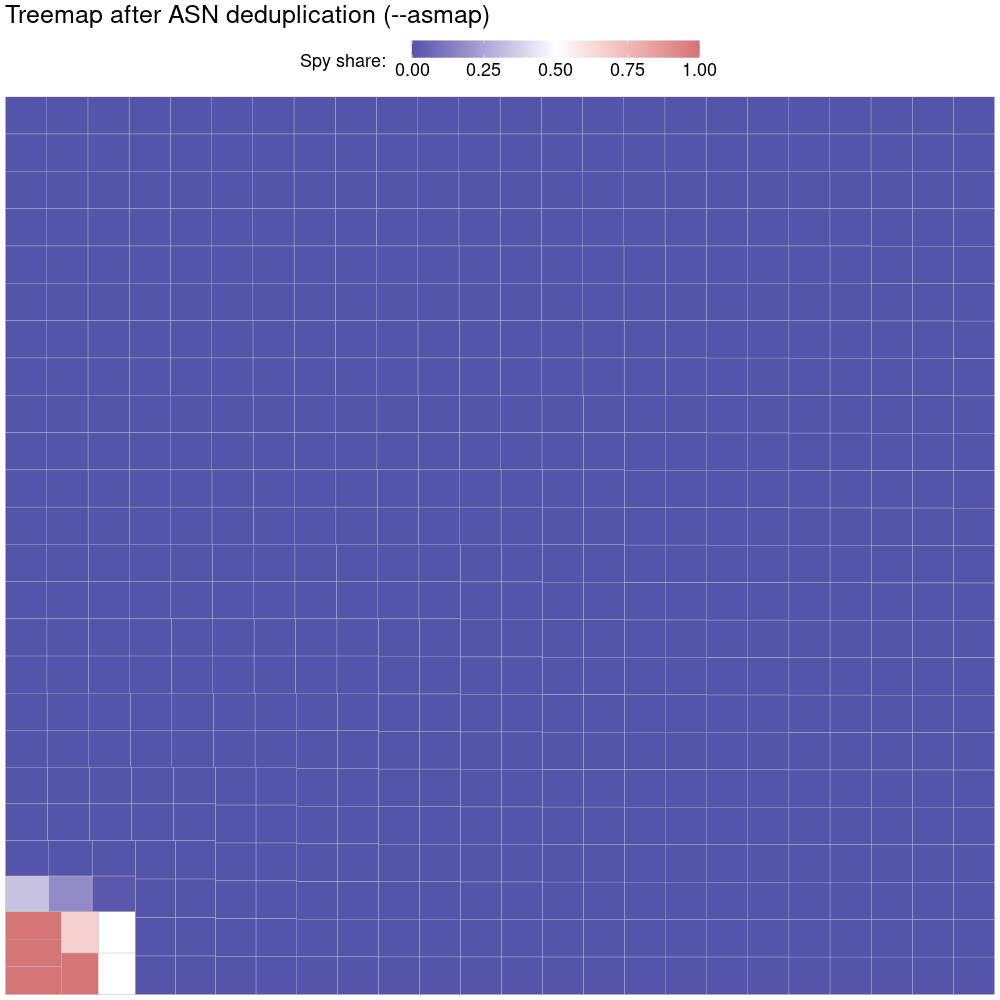
\includegraphics[width=0.49\linewidth]{images/treemap-asn-dedup}
\end{figure}

\section{Simulated effect on current suspected spy nodes}

The simulation is the one in \cite{Rucknium2025}, implemented by \texttt{gen.network()} in \texttt{xmrpeers} \cite{xmrpeers}, with one change: the subnet keys are replaced by a group key, so that the same function simulates /24 deduplication, AS deduplication, and the hybrid rule of Section \ref{sec:hybrid}. As in \cite{Rucknium2025}, every honest node, reachable or not, fills 12 outbound slots and then replaces a random connection 12 times; suspected spy nodes make no outbound connections; unreachable nodes are added so that 80 or 90 percent of honest nodes are unreachable; and peer list size limits are ignored. The faster draw used here was checked against the literal shuffle-and-deduplicate draw of \texttt{gen.network()}, and both agree with the analytical selection probability within sampling error (Appendix \ref{sec:appendix-draw}).

Table \ref{table-malicious-connection-summary} gives the number of outbound connections, out of 12, from honest nodes to suspected spy nodes. With 80 percent unreachable nodes, the mean in October 2026 is \simNewSubnetEightyMean{} (\simNewSubnetEightyPct{} percent) with /24 deduplication and \simNewAsmapEightyMean{} (\simNewAsmapEightyPct{} percent) with AS deduplication. For the May 2025 data the means are \simOldSubnetEightyMean{} and \simOldAsmapEightyMean{}; the /24 value reproduces the \simOldSubnetEightyMean{} connections (\simOldSubnetEightyPct{} percent) that \cite{Rucknium2025} reports for subnet deduplication on the same data, which validates the port of the simulation.

\begin{table}[t]
\caption{
{\fontsize{20}{25}\selectfont  Summary statistics: Number of outbound connections, out of 12, to suspected spy nodes}
} 
\begin{tabular*}{\linewidth}{@{\extracolsep{\fill}}lrrrrrrr}
\toprule
Scenario & N honest nodes & Min. & 1st Qu. & Median & Mean & 3rd Qu. & Max. \\ 
\midrule\addlinespace[2.5pt]
Oct 2026, /24 dedup, 80\% unreachable & 18,622 & 0 & 3 & 4 & 4.35 & 5 & 11 \\ 
Oct 2026, AS dedup, 80\% unreachable & 18,622 & 0 & 0 & 0 & 0.13 & 0 & 3 \\ 
Oct 2026, hybrid, 80\% unreachable & 18,622 & 0 & 0 & 1 & 0.78 & 1 & 4 \\ 
Oct 2026, /24 dedup, 90\% unreachable & 38,537 & 0 & 3 & 4 & 4.35 & 5 & 11 \\ 
Oct 2026, AS dedup, 90\% unreachable & 38,537 & 0 & 0 & 0 & 0.13 & 0 & 3 \\ 
Oct 2026, hybrid, 90\% unreachable & 38,537 & 0 & 0 & 1 & 0.78 & 1 & 4 \\ 
May 2025, /24 dedup, 80\% unreachable & 21,192 & 0 & 0 & 1 & 1.06 & 2 & 7 \\ 
May 2025, AS dedup, 80\% unreachable & 21,192 & 0 & 0 & 0 & 0.09 & 0 & 3 \\ 
May 2025, hybrid, 80\% unreachable & 21,192 & 0 & 0 & 0 & 0.56 & 1 & 4 \\ 
May 2025, /24 dedup, 90\% unreachable & 44,227 & 0 & 0 & 1 & 1.05 & 2 & 7 \\ 
May 2025, AS dedup, 90\% unreachable & 44,227 & 0 & 0 & 0 & 0.09 & 0 & 3 \\ 
May 2025, hybrid, 90\% unreachable & 44,227 & 0 & 0 & 0 & 0.56 & 1 & 4 \\ 
\bottomrule
\end{tabular*}
\label{table-malicious-connection-summary}
\end{table}


\subsection{Inbound connections\label{sec:inbound}}

Connections that no longer go to suspected spy nodes go to honest reachable nodes instead, and AS deduplication also moves connections from honest nodes in densely populated ASNs to honest nodes in sparsely populated ones (concern 4). Table \ref{table-inbound-summary} gives the distribution of inbound connections of honest reachable nodes, and Table \ref{table-inbound-by-asn-size} and Figure \ref{fig:inbound-by-k} split it by the number of honest reachable nodes in the node's AS. \ikSingleAsesPct{} percent of the ASes with honest reachable nodes contain only one. With AS deduplication every AS receives about the same share of inbound connections, which its nodes divide between them: a node receives about \inAloneAsmap{} inbound connections alone in its AS, \ikTwoAsmap{} with one other honest node, \ikThreeAsmap{} with two and \ikFourAsmap{} with three. With /24 deduplication most nodes receive about \inAloneSubnet{}. The \ikMoreNodes{} nodes (\ikMorePct{} percent) in ASes with up to \ikMoreMaxK{} honest nodes therefore receive more inbound connections than today, and the others fewer. Figure \ref{fig:inbound-share} shows where the inbound connections go. Nodes alone in their AS are \ishAloneNodes{} percent of honest reachable nodes; they receive \ishAloneMaster{} percent of all inbound connections with /24 deduplication and \ishAloneAsmap{} percent with AS deduplication. Nodes in ASes with ten or more honest nodes are \ishBigNodes{} percent of the nodes and receive \ishBigMaster{} percent and \ishBigAsmap{} percent. The live instances of Section \ref{sec:live} show the same shift on the real network: of their honest outbound peers, \lpAloneDefault{} percent were alone in their AS for default instances and \lpAloneAsmap{} percent for instances with \texttt{--asmap}, and \lpBigDefault{} and \lpBigAsmap{} percent were in ASes with ten or more honest nodes (\lpPeersDefault{} and \lpPeersAsmap{} peers; replication code: \texttt{live\_peer\_classes.py}). The live shift is smaller than simulated because real nodes choose from peer lists in which large-AS nodes are over-represented. The cause is the group draw: a node alone in its AS is drawn as often as a whole AS of hundreds of nodes. An adversary node alone in its AS is drawn as often too, which is the AS-distinct strategy analysed in Section \ref{sec:game}.

\begin{table}[t]
\caption{
{\fontsize{20}{25}\selectfont  Summary statistics: Number of inbound connections to honest reachable nodes}
} 
\begin{tabular*}{\linewidth}{@{\extracolsep{\fill}}lrrrrrrr}
\toprule
Scenario & N honest reachable nodes & Min. & 1st Qu. & Median & Mean & 3rd Qu. & Max. \\ 
\midrule\addlinespace[2.5pt]
Oct 2026, /24 dedup, 80\% unreachable & 2,690 & 0 & 24 & 67 & 52.94 & 75.75 & 110 \\ 
Oct 2026, AS dedup, 80\% unreachable & 2,690 & 0 & 1 & 7 & 82.19 & 105 & 452 \\ 
Oct 2026, hybrid, 80\% unreachable & 2,690 & 0 & 9 & 81 & 77.64 & 140 & 190 \\ 
Oct 2026, /24 dedup, 90\% unreachable & 2,690 & 0 & 49.25 & 142 & 109.58 & 155 & 198 \\ 
Oct 2026, AS dedup, 90\% unreachable & 2,690 & 0 & 2 & 14 & 170.04 & 214 & 877 \\ 
Oct 2026, hybrid, 90\% unreachable & 2,690 & 0 & 20 & 165 & 160.69 & 291 & 362 \\ 
May 2025, /24 dedup, 80\% unreachable & 2,764 & 4 & 79 & 87 & 83.87 & 93 & 121 \\ 
May 2025, AS dedup, 80\% unreachable & 2,764 & 0 & 7 & 37 & 91.32 & 133.25 & 372 \\ 
May 2025, hybrid, 80\% unreachable & 2,764 & 4 & 75 & 96 & 87.71 & 106 & 140 \\ 
May 2025, /24 dedup, 90\% unreachable & 2,764 & 11 & 171 & 182 & 175.16 & 191 & 227 \\ 
May 2025, AS dedup, 90\% unreachable & 2,764 & 0 & 14 & 78 & 190.59 & 256.5 & 738 \\ 
May 2025, hybrid, 90\% unreachable & 2,764 & 13 & 157 & 204 & 182.99 & 220 & 272 \\ 
\bottomrule
\end{tabular*}
\label{table-inbound-summary}
\end{table}


\begin{table}[t]
\caption{
{\fontsize{20}{25}\selectfont  Inbound connections of honest reachable nodes by the number of honest reachable nodes in their AS} \\ 
{\fontsize{14}{17}\selectfont  October 2026, 90 percent unreachable. Median: inbound connections per node. Share: percent of all inbound connections of honest reachable nodes}
} 
\begin{tabular*}{\linewidth}{@{\extracolsep{\fill}}rrrrrrr}
\toprule
Honest nodes in AS & ASes & Nodes (pct) & /24: median & AS: median & /24: share (pct) & AS: share (pct) \\ 
\midrule\addlinespace[2.5pt]
1 & 357 & 357 (13) & 151 & 801 & 18.2 & 62.3 \\ 
2 & 90 & 180 (7) & 148 & 402.5 & 8.7 & 15.8 \\ 
3 & 37 & 111 (4) & 150 & 267 & 5.5 & 6.5 \\ 
4 & 29 & 116 (4) & 150 & 200 & 5.5 & 5.1 \\ 
5-9 & 37 & 239 (9) & 150 & 120 & 11.5 & 6.5 \\ 
10-49 & 17 & 328 (12) & 149 & 40.5 & 15.2 & 2.9 \\ 
50-199 & 4 & 445 (17) & 26 & 6 & 10.5 & 0.7 \\ 
200+ & 2 & 914 (34) & 71 & 1 & 24.9 & 0.2 \\ 
\bottomrule
\end{tabular*}
\label{table-inbound-by-asn-size}
\end{table}


\begin{figure}[H]
\caption{Median inbound connections per honest reachable node, by the number of honest reachable nodes in its AS, October 2026, 90 percent unreachable nodes}
\label{fig:inbound-by-k}
\centering{}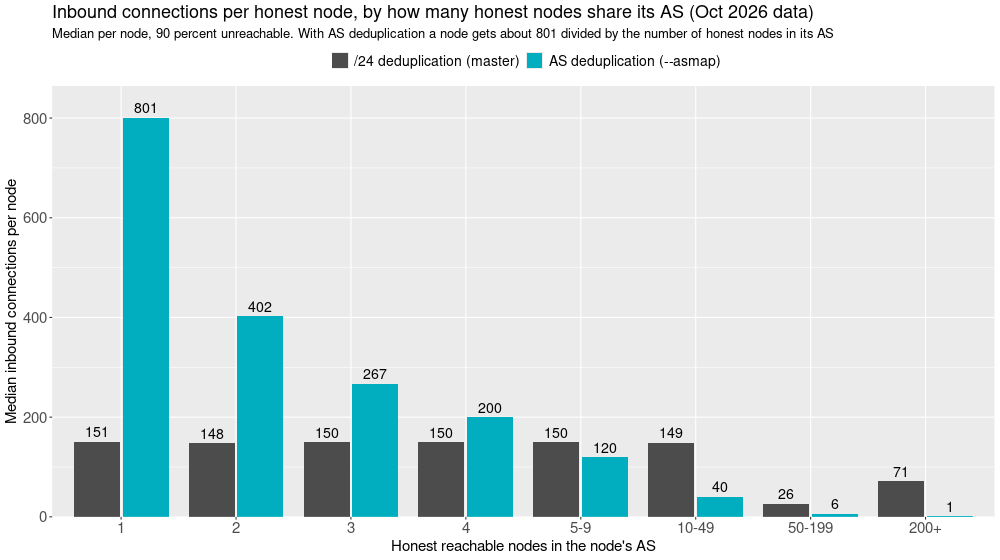
\includegraphics[scale=0.45]{images/inbound-by-k}
\end{figure}

\begin{figure}[H]
\caption{Share of honest reachable nodes and share of their inbound connections, by the number of honest reachable nodes in the node's AS, October 2026, 90 percent unreachable nodes}
\label{fig:inbound-share}
\centering{}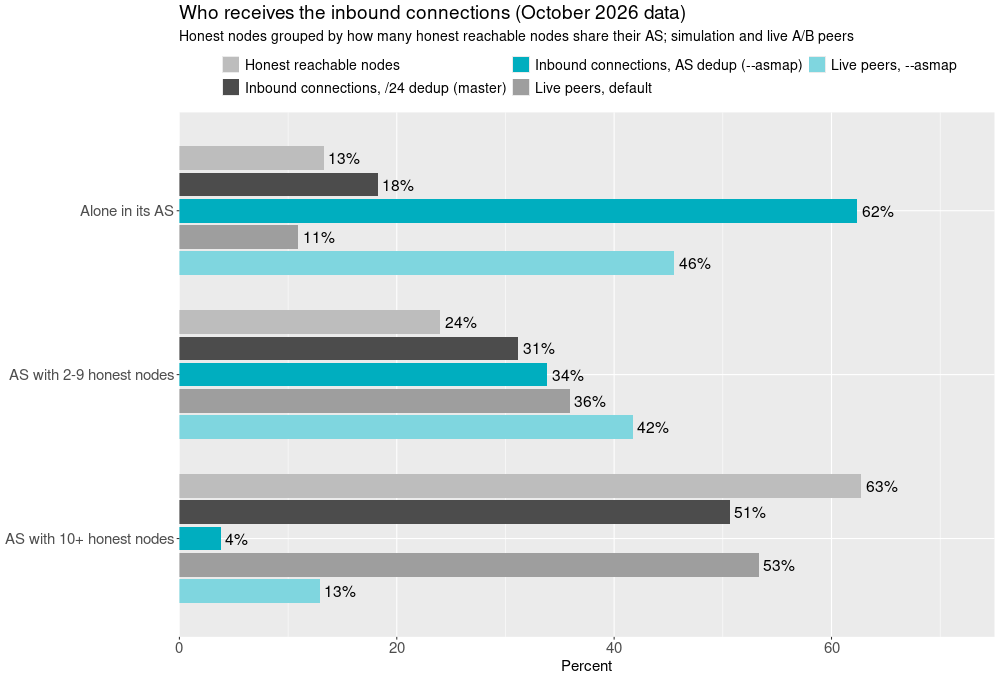
\includegraphics[scale=0.45]{images/inbound-share}
\end{figure}


\section{Protocol-adversary interaction as a game\label{sec:game}}

The simulation above holds the adversary's behaviour fixed. As in Section 4 of \cite{Rucknium2025}, we now let the adversary respond, and ask under what conditions AS deduplication is better for honest nodes than /24 deduplication. We make the assumptions of \cite{Rucknium2025}: the privacy impact is the probability that a single draw selects an adversary node; costs are linear in the number of nodes; and the adversary uses one strategy at a time. In addition we assume that the adversary does not place nodes in groups that contain honest nodes, which is the adversary's best use of a node when every group costs the same and the adversary obtains less than about half of the draws (Appendix \ref{sec:appendix-shared}).

The protocol chooses /24 deduplication ($24$) or AS deduplication ($A$). The adversary chooses between:
\begin{itemize}
\item \emph{bulk}: nodes in distinct /24 subnets inside few ASes, for example virtual servers from one cloud provider, at price $w_{24}$ per node and occupying $m$ ASNs;
\item \emph{AS-distinct}: one node in each of many ASes, at price $w_{A}$ per node. Each such node is also in a distinct /24 subnet.
\end{itemize}
Let $H_{24}$ and $H_{A}$ be the numbers of distinct /24 subnets and ASNs that contain at least one honest reachable node, and $b$ the adversary's budget. Following the derivation of equations (1) and (2) of \cite{Rucknium2025}:
\begin{align}
p_{24,\mathrm{bulk}} &= \frac{b}{w_{24}H_{24}+b} & p_{24,\mathrm{AS}} &= \frac{b}{w_{A}H_{24}+b}\label{eq:p24}\\
p_{A,\mathrm{bulk}} &\le \frac{m}{H_{A}+m} & p_{A,\mathrm{AS}} &= \frac{b}{w_{A}H_{A}+b}\label{eq:pA}
\end{align}
$p_{A,\mathrm{bulk}}$ does not depend on the budget: however many nodes the adversary puts in its $m$ ASes, they are $m$ groups.

\begin{prop}
Assume $w_{24} \le w_{A}$, so that the bulk strategy is the adversary's best response to /24 deduplication. The probability that a draw selects an adversary node is lower under AS deduplication against the AS-distinct strategy than under /24 deduplication against the bulk strategy, $p_{A,\mathrm{AS}} < p_{24,\mathrm{bulk}}$, if and only if
\begin{equation}
\frac{w_{A}}{w_{24}} > \frac{H_{24}}{H_{A}}.\label{eq:threshold}
\end{equation}
\end{prop}
The proof is the same as for inequality (3) of \cite{Rucknium2025}. For a fixed price, AS deduplication is worse against the AS-distinct strategy than /24 deduplication is, $p_{A,\mathrm{AS}} > p_{24,\mathrm{AS}}$, because $H_{A} < H_{24}$. This is concern 2: honest nodes concentrated in a few server-provider ASes count as few groups, and each adversary node in its own AS counts as a full group. Inequality (\ref{eq:threshold}) quantifies it. With the October 2026 data $H_{24}/H_{A} = \hTwentyFourNew/\hAsnNew = \thresholdNew$, and with the May 2025 data $\hTwentyFourOld/\hAsnOld = \thresholdOld$. If the adversary can find as many distinct ASes as it has nodes, AS deduplication is the better default only if a node in a distinct AS costs about three and a half times as much as a node in a distinct /24 subnet. The price survey and Section \ref{sec:response} below show that the price condition fails, and that the number of available ASes is what limits the adversary.

\subsection{Prices}

\textbf{Bulk.} $w_{24}$ is low for the bulk strategy observed in October 2026. The cheapest virtual server of the provider that hosts \spyTopAsnPctNew{} percent of the suspected spy nodes, AS\spyTopAsnNew{}, costs USD 4.00 per month and includes a public IPv4 address \cite{DOPricing}. The \spyTopAsnNNew{} suspected spy nodes in that AS are in \spyTwentyFourNew{} distinct /24 subnets in total (Table \ref{table-concentration}), so distinct /24 subnets come at almost no premium.

\textbf{Own ASN.} An adversary can register its own ASN, which costs EUR 50 per year at the RIPE NCC plus EUR 1,800 per year for an LIR account \cite{RIPE848}, and it must announce at least a /24 subnet, for which \cite{Rucknium2025} cites leasing prices of USD 118 to 250 per month. This is about thirty times the price of a USD 4 virtual server, well above the threshold (\ref{eq:threshold}).

\textbf{Rented servers in other ASes.} The cheaper way to occupy a distinct AS is to rent a server from another hosting provider. Table \ref{table-prices} lists the cheapest plan with a public IPv4 address of \nPriceProviders{} hosting providers that host honest reachable Monero nodes in the October 2026 data, taken from their pricing pages \cite{PricePages,DOPricing}, with EUR prices converted at the European Central Bank reference rate \cite{ECB20261005}. They cover \nPriceAsns{} distinct ASNs, because one provider (Contabo) operates three regional ASNs. All \nPriceAsns{} cost between USD \priceMin{} and \priceMax{} per month, at most \priceMaxRatio{} times the USD 4.00 bulk price, far below the threshold of \thresholdNew. Price alone therefore does not protect AS deduplication: an adversary can obtain distinct ASes at nearly the bulk price. Pricing pages of some other providers that host honest nodes (Vultr, Akamai/Linode) refused automated access, and Hetzner's page renders its prices with JavaScript, so they are not in the table; Hetzner charges EUR 0.50 per month extra for a primary IPv4 address \cite{HetznerIPv4}.

\begin{table}[t]
\caption{
{\fontsize{20}{25}\selectfont  Cheapest plan with a public IPv4 address, by hosting provider} \\ 
{\fontsize{14}{17}\selectfont  Prices from the providers' pricing pages, accessed 2026-10-05. EUR converted at the ECB reference rate of 2026-10-05 (1.1204 USD/EUR)}
} 
\begin{tabular*}{\linewidth}{@{\extracolsep{\fill}}llllrr}
\toprule
Provider & ASN & Plan & List price & USD/month & Honest nodes in ASN \\ 
\midrule\addlinespace[2.5pt]
InterServer & AS19318 & 1 Slice & 3.00 USD & 3.00 & 8 \\ 
DigitalOcean & AS14061 & Basic Droplet 512 MiB 1 vCPU 10 GiB & 4.00 USD & 4.00 & 630 \\ 
OVHcloud & AS16276 & VPS-1 & 4.54 USD & 4.54 & 284 \\ 
Contabo & AS51167 & Cloud VPS & 4.40 EUR & 4.93 & 46 \\ 
Contabo Asia & AS141995 & Cloud VPS & 4.40 EUR & 4.93 & 14 \\ 
Contabo US & AS40021 & Cloud VPS & 4.40 EUR & 4.93 & 5 \\ 
Amazon Lightsail & AS16509 & Linux bundle with public IPv4 & 5.00 USD & 5.00 & 9 \\ 
IONOS & AS8560 & VPS S+ & 6.00 USD & 6.00 & 7 \\ 
AlexHost & AS200019 & U1 & 6.00 EUR & 6.72 & 9 \\ 
\bottomrule
\end{tabular*}
\label{table-prices}
\end{table}


What limits the adversary is the \emph{number} of ASes in which it can rent servers. A spy node needs a public IPv4 address that accepts inbound connections, which in practice means a hosting provider rather than a residential network. The X4BNet community list of datacenter ASNs \cite{X4BDatacenter} contains \nDcList{} ASNs. Of the \hAsnNew{} ASNs with honest reachable nodes in October 2026, \nHonestDcAsn{} are on that list and hold \nHonestDcNodes{} of the \nHonestNew{} honest nodes; the other \nHonestNonDcAsn{} are mostly residential and access networks.

\subsection{Simulated adversary response\label{sec:response}}

The payoffs above use a single draw. To include the 12 outbound slots and the churn, the simulation of the previous section was repeated with the observed suspected spy nodes replaced by synthetic adversary fleets. Only the honest reachable nodes are simulated as originators; unreachable honest nodes would add originators with the same distribution of outbound connections.

\textbf{Price premium.} The fleet is replaced by $\lfloor n_{\mathrm{spy}}\, w_{24}/w_{A} \rfloor$ nodes, each in its own new AS and /24 subnet, for price premiums $w_{A}/w_{24}$ of 1, 2, 3.46, 5 and 10, where $n_{\mathrm{spy}}$ is the number of suspected spy nodes in the dataset (Table \ref{table-response}; replication code: \texttt{response\_sim.R}). With no premium, the adversary obtains \respAsmapROneNew{} of 12 connections under AS deduplication, compared with \respSubnetROneNew{} under /24 deduplication (October 2026 data; May 2025: \respAsmapROneOld{} and \respSubnetROneOld{}). This confirms concern 1 under the assumption that the adversary can find as many distinct ASes as it has nodes.

\begin{table}[t]
\caption{
{\fontsize{20}{25}\selectfont  Mean outbound connections, out of 12, to adversary nodes when the adversary responds}
} 
\begin{tabular*}{\linewidth}{@{\extracolsep{\fill}}llrrrr}
\toprule
Data & Adversary & Adversary nodes & /24 dedup & AS dedup & Hybrid \\ 
\midrule\addlinespace[2.5pt]
Oct 2026 & Observed suspected spy nodes & 1293 & 4.38 & 0.13 & 0.80 \\ 
Oct 2026 & AS-distinct, wA/w24 = 1 & 1293 & 4.71 & 8.31 & 5.32 \\ 
Oct 2026 & AS-distinct, wA/w24 = 2 & 646 & 2.95 & 6.34 & 3.48 \\ 
Oct 2026 & AS-distinct, wA/w24 = 3.46 & 373 & 1.90 & 4.73 & 2.34 \\ 
Oct 2026 & AS-distinct, wA/w24 = 5 & 258 & 1.37 & 3.70 & 1.75 \\ 
Oct 2026 & AS-distinct, wA/w24 = 10 & 129 & 0.71 & 2.22 & 0.93 \\ 
May 2025 & Observed suspected spy nodes & 1843 & 1.05 & 0.09 & 0.56 \\ 
May 2025 & AS-distinct, wA/w24 = 1 & 1843 & 4.92 & 8.37 & 5.15 \\ 
May 2025 & AS-distinct, wA/w24 = 2 & 921 & 3.07 & 6.41 & 3.32 \\ 
May 2025 & AS-distinct, wA/w24 = 3.46 & 532 & 1.99 & 4.81 & 2.20 \\ 
May 2025 & AS-distinct, wA/w24 = 5 & 368 & 1.47 & 3.80 & 1.63 \\ 
May 2025 & AS-distinct, wA/w24 = 10 & 184 & 0.81 & 2.31 & 0.88 \\ 
\bottomrule
\end{tabular*}
\label{table-response}
\end{table}


\textbf{Limited supply of ASes.} The more realistic constraint is the number of rentable ASes, $K$. The fleet of \nSpyNew{} nodes, each in its own /24 subnet, is spread evenly over $K$ datacenter ASNs at an equal price per node, which Table \ref{table-prices} shows is approximately true for the cheapest providers. $K$ is set to the \nPriceAsns{} ASNs of Table \ref{table-prices}, to the \nHonestDcAsn{} datacenter ASNs that host honest reachable nodes, to all \nDcList{} listed datacenter ASNs, and to intermediate values made of the \nHonestDcAsn{} plus randomly chosen other listed ASNs (replication code: \texttt{supply\_sim.R}). Adversary nodes in an AS that also hosts honest nodes share that AS's group, as in the real network. Table \ref{table-supply} and Figure \ref{fig:supply} give the results. AS deduplication gives fewer connections to the adversary than /24 deduplication as long as the adversary can rent servers in fewer than about \kBreakEven{} ASes: \supAsmapKIX{} connections with $K=\nPriceAsns$, \supAsmapKXCIX{} with $K=\nHonestDcAsn$, against \supSubnetKIX{} with /24 deduplication. With $K=\nDcList$ the adversary obtains \supAsmapKCMXXXIII{} connections, more than with /24 deduplication. The break-even agrees with $k^{*}=\kStarNew{}$ from the single-draw model of Section \ref{sec:game}. Repeated with \beSeeds{} further random seeds on the four vantage machines, the break-even is \beMean{} ASes (standard deviation \beSd, range \beMin{} to \beMax). If a node in another AS costs more than a bulk node, the adversary can afford fewer nodes, but under AS deduplication only the number of ASes it occupies matters: with a price ratio of 1.5 and 1.75 the break-even, measured against the full bulk fleet under /24 deduplication, is \beRatioMid{} and \beRatioHigh{} ASes (replication code: \texttt{breakeven.R}).

\begin{table}[t]
\caption{
{\fontsize{20}{25}\selectfont  Mean outbound connections, out of 12, to adversary nodes spread over K ASNs}
} 
\begin{tabular*}{\linewidth}{@{\extracolsep{\fill}}rrrr}
\toprule
K & /24 deduplication (master) & AS deduplication (--asmap) & Hybrid \\ 
\midrule\addlinespace[2.5pt]
9 & 4.71 & 0.15 & 3.79 \\ 
99 & 4.71 & 1.61 & 5.23 \\ 
200 & 4.71 & 3.03 & 5.31 \\ 
300 & 4.71 & 4.09 & 5.32 \\ 
400 & 4.71 & 4.98 & 5.33 \\ 
600 & 4.71 & 6.21 & 5.32 \\ 
933 & 4.71 & 7.49 & 5.30 \\ 
\bottomrule
\end{tabular*}
\label{table-supply}
\end{table}


\begin{figure}[H]
\caption{Adversary connections when the adversary spreads over $K$ rentable ASNs}
\label{fig:supply}
\centering{}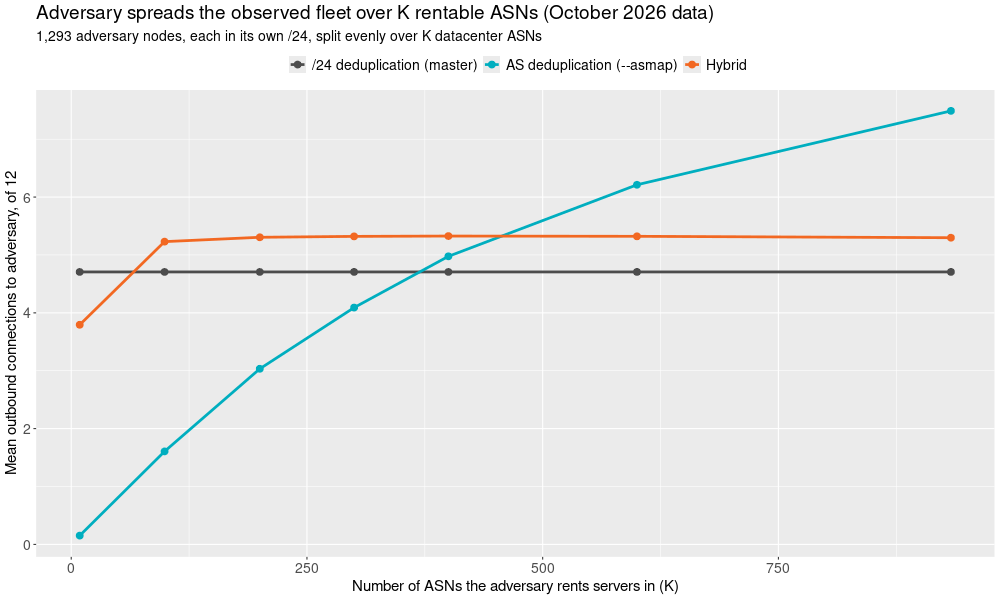
\includegraphics[scale=0.45]{images/supply}
\end{figure}

\subsection{Opt-in}

If few nodes use \texttt{--asmap}, the adversary's best response is to the protocol that most nodes use, /24 deduplication, so it keeps the bulk strategy. Nodes that opt in then face the observed fleet, against which AS deduplication gives \simNewAsmapEightyMean{} connections to suspected spy nodes out of 12, against \simNewSubnetEightyMean{} with /24 deduplication (Table \ref{table-malicious-connection-summary}). The other nodes are unaffected, apart from the change in inbound connections caused by the opted-in nodes. The result therefore supports AS deduplication as an opt-in option.

The argument assumes that few nodes opt in. The MRL ban list is also opt-in, yet \banAdoptPct{} percent of honest reachable nodes block it: their sampled white lists contain no ban-listed address, against a median of \banAdoptOthersPct{} percent for the other nodes (replication code: \texttt{ban\_adoption.py}; the method cannot distinguish the MRL list from a DNS blocklist that covers the same addresses). Because each node selects its outbound peers by its own rule, the number of ASes the adversary needs to offset AS deduplication, about \kBreakEven{}, does not depend on how many nodes opt in, and nodes that do not opt in are unaffected. Adoption changes the adversary's gain from spreading. If as many nodes opted in as block the ban list, spreading would win back most of the connections that AS deduplication removes, and for those nodes opt-in would become the default case of Section \ref{sec:feasibility}. The crawler measures the number of ASes the adversary uses continuously \cite{Observatory}. A rise from the current \spyAsnNew{} ASes towards the hundreds would be the signal to advise nodes to turn the option off.

\section{Can an adversary rent servers in about \kBreakEven{} ASes?\label{sec:feasibility}}

Section \ref{sec:response} reduces the question of a default to one number: the number $K$ of distinct ASes in which an adversary can rent servers with inbound-reachable public IPv4 addresses. This section collects the available evidence and estimates $K$ with a sample survey.

\subsection{What adversaries have done}

Every suspected spy fleet observed so far uses few ASes. The MRL ban list \cite{MRLBanList}, version 2, covers \banAddresses{} IPv4 addresses in \banAsns{} ASNs. The fingerprint-flagged reachable nodes of October 2026 are \nSpyNew{} addresses in \spyAsnNew{} ASNs, \spyTopAsnPctNew{} percent of them in one. A peer-list poisoning pool observed by the crawler is hosted by one proxy provider (PEG Tech); all addresses gossiped from that provider's ASNs, \pegIps{} in total, fall in \pegAsns{} ASNs. The hosting provider is not necessarily the operator. These adversaries chose bulk strategies against the status quo and /24 deduplication, which is their best response to those rules (Section \ref{sec:game}). Their behaviour shows what is cheapest today, not what they could do if AS deduplication became the default.

\subsection{Where outsiders run public servers}

A lower bound on $K$ is the number of ASes in which people other than the network operator already run inbound-reachable servers. Three networks give such counts, with addresses mapped to ASNs by the same asmap:
\begin{itemize}
\item Tor relays with an IPv4 address \cite{Onionoo}: \torAses{} ASes, of which \torDc{} are on the X4BNet datacenter list \cite{X4BDatacenter}.
\item Reachable Bitcoin nodes with an IPv4 address \cite{Bitnodes}: \btcAses{} ASes, of which \btcDc{} are on the list.
\item Reachable Monero nodes in October 2026: \hAsnNew{} ASes, of which \nHonestDcAsn{} are on the list.
\end{itemize}
Together they cover \unionAses{} ASes, \unionDc{} of them on the datacenter list. The Monero crawler also records every address that peers gossip: since \crawlStart, the four vantage points saw \crawlIps{} distinct public IPv4 addresses in \crawlAsns{} ASNs, of which \crawlReachIps{} addresses in \crawlReachAsns{} ASNs were reachable \cite{Observatory}.

The \unionDc{} datacenter-listed ASes are fewer than \kBreakEven, but the remaining \unionUnlisted{} ASes are not all residential. The datacenter list is community-maintained and incomplete: for example, AS40021 (Contabo's US network, Table \ref{table-prices}) and AS210083 (Privex), both of which host honest reachable Monero nodes, are not on it. Counting therefore does not decide whether $K$ exceeds \kBreakEven.

\subsection{Survey of rentable ASes}

$K$ was estimated by a random-sample survey of the \svFrame{} ASes that host public servers (replication code: \texttt{survey\_sample.py}, \texttt{survey\_fetch.py}, \texttt{survey\_verdicts.py}, \texttt{survey\_estimate.py}; saved copies of all pages in \texttt{data/survey/pages}).
\begin{enumerate}
\item A simple random sample of $n=\svn$ ASes was drawn with a fixed seed.
\item Each AS was matched to its PeeringDB record (name, website and network type) \cite{PeeringDB} and to the bgp.tools tags ``Server Hosting'', ``DSL'' and ``Mobile'' \cite{BgpToolsTags}. bgp.tools defines Server Hosting as a network that ``provides commercial hosting, colocation, VPS, etc services (other people can buy machines and exit traffic from this network)'', which is the property that matters here.
\item The website of each AS was fetched and searched, in several languages, for offers of virtual or dedicated servers and their monthly prices. Where a site blocked automated access, a third-party listing was used and marked as secondary evidence.
\item Each AS was classified as \emph{rentable} if it carries the Server Hosting tag or a server offer was found, \emph{not rentable} if it carries only access-network tags or is registered as a residential, education, research or media network and no server offer was found, and \emph{unknown} otherwise. Found evidence overrides tags.
\end{enumerate}

Of the \svn{} sampled ASes, \svR{} are rentable, \svN{} are not rentable and \svU{} are unknown (Appendix \ref{sec:appendix-survey}). Table \ref{table-survey-rentable} lists the rentable ones. A price was found for \svPriced{} of them, and \svCheap{} of those cost USD 7 per month or less, the range of Table \ref{table-prices}; for \svCheapV{} of the \svCheap{} the page states that an IPv4 address is included or gives its price. Prices in other currencies were converted at official reference rates \cite{FXRates,ECB20261005}.

\begin{table}[t]
\caption{
{\fontsize{20}{25}\selectfont  Sampled ASes classified as rentable\small } \\ 
{\fontsize{14}{17}\selectfont  IPv4: incl. = included, add-on = priced add-on included in the price, n/s = not stated. Src: P = provider page, S = third-party listing, T = bgp.tools tag only\small }
} 
\begin{tabular*}{\linewidth}{@{\extracolsep{\fill}}lllrll}
\toprule
ASN & Network & Evidence & USD/mo & IPv4 & Src \\ 
\midrule\addlinespace[2.5pt]
AS216071 & VDSINA & VDS/VPS from USD 2.10/month & 2.1 & n/s & P \\ 
AS215467 & Skhron & VPS EUR 1.69/month, IPv4 add-on EUR 0.65/m & 2.62 & add-on & P \\ 
AS7489 & HostUS & KVM VPS, 512 MB, USD 35/year, 1 IPv4 & 2.92 & incl. & S \\ 
AS202053 & UpCloud & Starter cloud server from USD 3.5/month, I & 3.5 & incl. & S \\ 
AS51290 & HosTeam & VPS Bronze 15.00 PLN/30d net, IPv4 + IPv6 & 3.84 & incl. & P \\ 
AS58212 & Dataforest & self-service cloud 'Seeds' from EUR 4.07/m & 4.56 & n/s & S \\ 
AS215590 & DpkgSoft International Lim & virtual servers from 459 RUB/month & 5.4 & n/s & P \\ 
AS34700 & Maxnet Ukraine & VPS 250 UAH/month, 1 IPv4 address & 5.55 & incl. & P \\ 
AS40244 & Turnkey Internet & VPS pro.sm.amd USD 10/month & 10.0 & n/s & P \\ 
AS206264 & Amarutu Technology Ltd. & VPS Medium Risk A USD 39.99/month & 39.99 & n/s & P \\ 
AS7296 & Alchemy Communications, In & bare metal servers, private cloud, colocat &  &  & S \\ 
AS21581 & M5 Computer Security / M5H & dedicated servers, bare metal, cloud insta &  &  & P \\ 
AS56030 & Voyager Internet & cloud servers / virtual data centre, coloc &  &  & P \\ 
AS42675 & Obehosting & dedicated servers and colocation, Stockhol &  &  & S \\ 
AS16302 & SuomiCommunications & bgp.tools tag Server Hosting &  &  & T \\ 
AS12310 & iNES Group & VPS and dedicated servers, price on reques &  &  & S \\ 
AS35366 & ISPpro Internet KG & vServer and dedicated root servers &  &  & S \\ 
AS208208 & CYBERSE & business cloud from 79 EUR/month, colocati &  &  & P \\ 
AS200303 & LUMASERV & vServer / cloud computing &  &  & P \\ 
AS42532 & Veesp SIA & VPS and dedicated servers &  &  & P \\ 
AS200950 & Calibour Limited & VPS and dedicated servers &  &  & P \\ 
AS45899 & VNPT & bgp.tools tag Server Hosting &  &  & T \\ 
AS399122 & VPS House Technology Group & VPS, cloud and dedicated servers &  &  & P \\ 
AS49791 & 3HCLOUD & shared vCPU server USD 1.5/month, IPv4 pri &  & extra & P \\ 
\bottomrule
\end{tabular*}
\label{table-survey-rentable}
\end{table}


With 95 percent Wilson confidence intervals, scaled to the \svFrame{} ASes of the frame:
\begin{itemize}
\item rentable ASes: \svKR{} (\svKRLoLo{} to \svKRHiHi{}); \svKRU{} (\svKRULoLo{} to \svKRUHiHi{}) if every unknown AS is rentable;
\item ASes confirmed rentable at USD 7 per month or less: \svKCheap{} (\svKCheapLoLo{} to \svKCheapHiHi{}), of which \svKCheapV{} (\svKCheapVLoLo{} to \svKCheapVHiHi{}) with an IPv4 address stated in the price.
\end{itemize}
The second estimate is a lower bound: a price was found for only \svPriced{} of the \svR{} rentable ASes in the sample, and \svCheap{} of those \svPriced{} are cheap. The global estimate assumes that every AS with the Server Hosting tag is rentable. Because tagged ASes were classified as rentable by rule, the survey does not test this assumption; for \svPriced{} of the tagged or otherwise rentable ASes a priced offer was found.

The frame contains only ASes in which Tor, Bitcoin or Monero servers already run, and an adversary is not limited to them. bgp.tools tags \svVpshTotal{} ASes as Server Hosting. In the sample the tag identified \svTaggedinSample{} of the \svR{} rentable ASes, a recall of \svTagRecall, which suggests that about \svKGlobalHosting{} ASes offer server hosting worldwide.

\textbf{Result.} The number of ASes in which servers can be rented is larger than the break-even of about \kBreakEven{}: \svKR{} (\svKRLoLo{} to \svKRHiHi) within the frame alone and about \svKGlobalHosting{} worldwide. The number confirmed to be as cheap as the bulk strategy is lower, \svKCheap{} within the frame, but that is a lower bound and \svCheap{} of the \svPriced{} rentable ASes with a price were that cheap. Price and supply therefore do not appear to prevent an adversary from spreading over more than \kBreakEven{} ASes. The constraints that remain are operational: an adversary that uses \kBreakEven{} providers manages \kBreakEven{} accounts, payment methods and abuse desks, and each provider can suspend its servers. These costs are not measured here.

\section{A complementary defence: AS-diverse Dandelion++ stems\label{sec:stem}}

The privacy loss that spy nodes cause is concentrated in the stem phase of Dandelion++, in which a node forwards its own transactions to one of its stem peers \cite{Fanti2018a}. Monero chooses \texttt{CRYPTONOTE\_DANDELIONPP\_STEMS} $=2$ stems per epoch uniformly at random, without replacement, from the node's outbound connections (\texttt{connection\_map} in \texttt{src/net/dandelionpp.cpp}). We consider a change to the stem choice only: draw the stems uniformly over the \emph{ASes} of the outbound connections, then a connection uniformly within the AS. Outbound peer selection, and therefore the network graph and inbound load, are unchanged.

Against a bulk fleet, the connections that a node has to the fleet's few ASes collapse into few stem candidates. Against an adversary with one node per AS, every adversary connection remains its own candidate, and only honest connections that share an AS are merged, so the adversary gains little. Table \ref{table-stem} gives the probability that a stem is an adversary node, computed exactly for each honest reachable node from its simulated outbound connections (replication code: \texttt{stem\_sim.R}). With /24 deduplication and the observed suspected spy nodes it falls from \stemObsCur{} to \stemObsDiv{} percent per stem, and the probability that either of the two stems is an adversary node falls from \stemObsAnyCur{} to \stemObsAnyDiv{} percent. For a node that does not use the ban list it falls from \stemBanCur{} to \stemBanDiv{} percent, and for the May 2025 data from \stemOldCur{} to \stemOldDiv{} percent. Against one adversary node per AS (\nSpyNew{} ASes, none shared with honest nodes), the worst case for every rule considered here, it rises from \stemWorstCur{} to \stemWorstDiv{} percent.

\begin{table}[t]
\caption{
{\fontsize{20}{25}\selectfont  Dandelion++ stem exposure: percent probability that a stem is an adversary node\small } \\ 
{\fontsize{14}{17}\selectfont  Stem: current = 2 stems uniformly from the outbound connections (src/net/dandelionpp.cpp). AS-diverse = stems drawn uniformly over the ASes of the outbound connections\small }
} 
\begin{tabular*}{\linewidth}{@{\extracolsep{\fill}}lllrrr}
\toprule
Data & Adversary & Outbound & Spy/12 & Stem cur. & Stem AS-div. \\ 
\midrule\addlinespace[2.5pt]
Oct 2026 & Observed & AS & 0.1 & 1.1 & 1.1 \\ 
Oct 2026 & Observed & /24 & 4.4 & 36.5 & 12.3 \\ 
Oct 2026 & Observed + ban-list nodes & AS & 0.2 & 1.3 & 1.3 \\ 
Oct 2026 & Observed + ban-list nodes & /24 & 4.5 & 37.5 & 13.9 \\ 
Oct 2026 & Spread, 99 ASes & AS & 1.6 & 13.4 & 13.4 \\ 
Oct 2026 & Spread, 99 ASes & /24 & 4.7 & 39.2 & 41.9 \\ 
Oct 2026 & Spread, 370 ASes & AS & 4.8 & 39.7 & 39.7 \\ 
Oct 2026 & Spread, 370 ASes & /24 & 4.7 & 39.2 & 42.3 \\ 
Oct 2026 & Spread, 933 ASes & AS & 7.5 & 62.4 & 62.4 \\ 
Oct 2026 & Spread, 933 ASes & /24 & 4.7 & 39.2 & 42.4 \\ 
Oct 2026 & One node per AS & AS & 8.3 & 69.3 & 69.3 \\ 
Oct 2026 & One node per AS & /24 & 4.7 & 39.2 & 42.5 \\ 
Oct 2026 & 10 largest honest ASes & AS & 0.1 & 1.1 & 1.1 \\ 
Oct 2026 & 10 largest honest ASes & /24 & 4.7 & 39.2 & 36.7 \\ 
Oct 2026 & 30 largest honest ASes & AS & 0.4 & 3.2 & 3.2 \\ 
Oct 2026 & 30 largest honest ASes & /24 & 4.7 & 39.2 & 40.4 \\ 
Oct 2026 & Honest AS distribution & AS & 2.7 & 22.8 & 22.8 \\ 
Oct 2026 & Honest AS distribution & /24 & 4.7 & 39.2 & 38.0 \\ 
May 2025 & Observed & AS & 0.1 & 0.8 & 0.8 \\ 
May 2025 & Observed & /24 & 1.1 & 8.8 & 6.2 \\ 
\bottomrule
\end{tabular*}
\label{table-stem}
\end{table}


Figure \ref{fig:stem-spread} shows how quickly each rule loses its advantage as the adversary spreads. AS-diverse stems lose theirs early: spread over the \nHonestDcAsn{} datacenter ASes that host honest nodes, the adversary already obtains \stemNineNineDiv{} percent per stem, and further spreading adds less than one percentage point. AS deduplication of outbound connections keeps its advantage longer (\stemNineNineAsmap{} percent at \nHonestDcAsn{} ASes) but loses it at about \kBreakEven{} ASes (\stemThreeSeventyAsmap{} percent) and keeps deteriorating, to \stemWorstAsmap{} percent. No rule considered here is better than the current one against every adversary placement: a rule that trusts AS diversity tells the adversary which placement it trusts. The rules differ in what they lose in their worst case. AS-diverse stems lose at most \stemRegretDiv{} percentage points against the current rule and gain \stemObsGain{} against the observed fleet; AS deduplication of outbound connections has no comparable bound.

\begin{figure}[H]
\caption{Probability that a Dandelion++ stem is an adversary node as the adversary spreads its nodes over more ASes, October 2026}
\label{fig:stem-spread}
\centering{}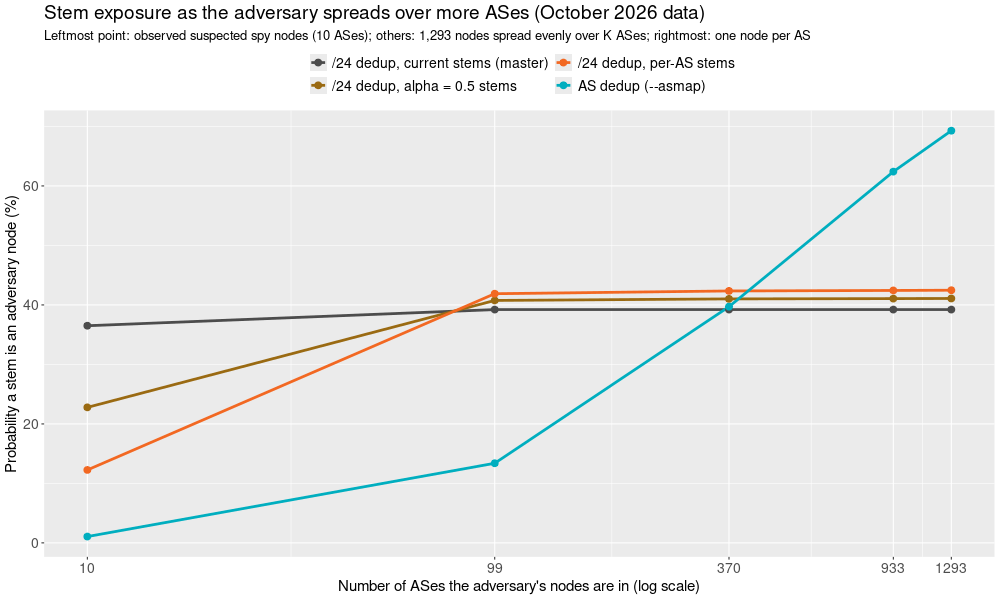
\includegraphics[scale=0.45]{images/stem-spread}
\end{figure}

The trade-off can be tuned by weighting each connection by $n^{-\alpha}$, where $n$ is the number of the node's outbound connections in the same AS: $\alpha=0$ is the current rule and $\alpha=1$ the AS-diverse rule (Table \ref{table-stem-alpha}). The worst-case cost grows slowly with $\alpha$ and the benefit against the observed fleet quickly: with $\alpha=0.5$ the stem exposure is \stemObsAlpha{} percent against the observed fleet and \stemWorstAlpha{} percent in the worst case, at most \stemRegretAlpha{} percentage points above the current rule.

\begin{table}[t]
\caption{
{\fontsize{20}{25}\selectfont  Stem exposure (percent) with connections weighted by n\textasciicircum{}(-alpha), /24 deduplication, October 2026\small }
} 
\begin{tabular*}{\linewidth}{@{\extracolsep{\fill}}crr}
\toprule
Weight exponent alpha & One node per AS & Observed suspected spy nodes \\ 
\midrule\addlinespace[2.5pt]
0 & 39.2 & 36.5 \\ 
0.25 & 40.2 & 29.5 \\ 
0.5 & 41.1 & 22.8 \\ 
0.75 & 41.8 & 17.0 \\ 
1 & 42.5 & 12.3 \\ 
\bottomrule
\end{tabular*}
\label{table-stem-alpha}
\end{table}


\textbf{Stem load.} AS-diverse stems move stem traffic towards honest nodes that are alone in their AS, the stem counterpart of concern 4. Table \ref{table-stemload} gives the expected stem traffic each honest reachable node receives. Against the observed suspected spy nodes the median rises from \loadMedCur{} to \loadMedDiv, partly because traffic that went to spy nodes now goes to honest ones; the maximum rises from \loadMaxCur{} to \loadMaxDiv, the Gini coefficient from \loadGiniCur{} to \loadGiniDiv, and nodes alone in their AS receive \loadAloneDiv{} instead of \loadAloneCur. The concentration is moderate compared with the inbound concentration of AS deduplication of outbound connections (Section \ref{sec:inbound}).

\begin{table}[t]
\caption{
{\fontsize{20}{25}\selectfont  Expected stem traffic received per honest reachable node, /24 deduplication, October 2026\small } \\ 
{\fontsize{14}{17}\selectfont  Sum over originators of the probability that the node is chosen as a stem. cur. = current rule, div. = AS-diverse. Alone: only honest reachable node in its AS\small }
} 
\begin{tabular*}{\linewidth}{@{\extracolsep{\fill}}lrrrrrrrr}
\toprule
Adversary & Med. cur. & Med. div. & Max cur. & Max div. & Gini cur. & Gini div. & Alone cur. & Alone div. \\ 
\midrule\addlinespace[2.5pt]
One node per AS & 0.75 & 0.64 & 1.92 & 2.03 & 0.29 & 0.33 & 0.83 & 0.89 \\ 
Observed + ban-list & 0.75 & 1.00 & 2.00 & 3.49 & 0.29 & 0.40 & 0.87 & 1.47 \\ 
Observed & 0.75 & 1.03 & 1.83 & 3.10 & 0.29 & 0.40 & 0.86 & 1.45 \\ 
\bottomrule
\end{tabular*}
\label{table-stemload}
\end{table}


\textbf{Adversaries aimed at the stem rule.} An adversary that knows the stem rule might place its nodes in the ASes that hold the most honest nodes, so that honest connections are merged with its own. With the observed fleet size, concentrating in the 10 or 30 largest honest ASes, or copying the honest AS distribution, gives \stemTopTenDiv{}, \stemTopThirtyDiv{} and \stemMimicDiv{} percent per stem (Table \ref{table-stem}), all below the one-node-per-AS case of \stemWorstDiv{} percent.

AS-diverse stems are not part of pull request \#11474. They need the asmap but no change to peer selection, so they could be used with /24 deduplication by every node that loads the map. Their effect on the anonymity guarantees of Dandelion++, which assume random stem choice among outbound connections, should be reviewed before they are adopted.

\section{Selection from real peer lists\label{sec:peerlists}}

The simulations above follow \cite{Rucknium2025} in letting every node choose from all reachable nodes. Real nodes choose from a white list of at most 1,000 and a gray list of at most 5,000 addresses, built from the peer lists of their neighbours, and prefer recently seen white-list entries. That model predicted 30.8 percent of outbound connections to suspected spy nodes for the status quo in May 2025 \cite{Rucknium2025}, while \cite{Kopyciok2026} measured 6.69 to 7.78 percent on default nodes in June 2025. Absolute shares from the uniform model are therefore probably too high.

To use real candidate pools, each of the \plNodes{} honest reachable nodes that completed a handshake was asked four times, from the four vantage points, for its peer list; each response is a random sample of up to 250 white-list entries (replication code: \texttt{pl\_crawl.py}). On average \plListSpy{} percent of a node's entries are suspected spy nodes or reachable ban-listed nodes, close to the 16.22 percent of peer-list entries that \cite{Kopyciok2026} attribute to one AS; \plUnknown{} percent are addresses not known to be reachable, which are treated as failed connection attempts. Each node then selects outbound connections from its own list with the algorithm of \texttt{make\_new\_connection\_from\_peerlist()}: deduplication by group, sorting by \texttt{last\_seen}, the first 20 untried candidates, and the cubic preference for recent entries of \texttt{get\_random\_index\_with\_fixed\_probability()} (replication code: \texttt{pl\_sim.py}). Only the white list is modelled; monerod draws about 70 percent of outbound connections from it (\texttt{P2P\_DEFAULT\_WHITELIST\_CONNECTIONS\_PERCENT}).

Table \ref{table-peerlists} gives the results. With /24 deduplication and no ban list, \plSubnetObs{} of 12 outbound connections go to suspected spy nodes, fewer than in the uniform model, and AS deduplication reduces this to \plAsmapObs. In the spread case the same list entries are relabelled so that every adversary node is in its own AS, the most favourable placement for the adversary; AS deduplication then gives \plAsmapSpr{} connections against \plSubnetSpr{} with /24 deduplication, a smaller penalty than in the uniform model.

\textbf{AS-aware peer lists.} Peer-list poisoning is the mechanism that gives the adversary its share of candidates \cite{Kopyciok2026}, who suggest pruning duplicated subnets or ASes from peer lists. Bitcoin Core applies the asmap to the same problem: it uses the AS to place addresses in its address manager's buckets, which limits the share of the address table that one AS can occupy \cite{BitcoinPR16702}. Monero's white and gray lists have no such limit. Capping each AS at 3.1 percent of a node's list, the fraction of Bitcoin's tried table that one group can occupy (8 of 256 buckets \cite{BitcoinAddrman}), with /24 deduplication otherwise unchanged, reduces the connections to the observed suspected spy nodes from \plSubnetObs{} to \plCapThreeObs, and a 1 percent cap to \plCapOneObs. Against the spread case the cap gives \plCapThreeSpr{} and \plCapOneSpr{} connections, against \plSubnetSpr, because capping the large honest ASes raises the adversary's share of what remains. The cap is applied here to a static list; a cap applied when entries are inserted, as in Bitcoin, may behave differently and should be simulated with list dynamics.

\begin{table}[t]
\caption{
{\fontsize{20}{25}\selectfont  Outbound selection from real peer lists\small } \\ 
{\fontsize{14}{17}\selectfont  Each honest reachable node selects from the white-list entries it returned in four handshakes. Spread: the same entries, one AS per adversary node. Cap: per-AS cap on list entries\small }
} 
\begin{tabular*}{\linewidth}{@{\extracolsep{\fill}}lllrrrr}
\toprule
Adversary & Ban & Strategy & List spy \% & Spy/12 & Stem cur. \% & Stem AS-div. \% \\ 
\midrule\addlinespace[2.5pt]
Observed & off & AS & 17.5 & 0.71 & 5.9 & 5.9 \\ 
Observed & off & AS + cap 1.0\% & 1.5 & 0.24 & 2.0 & 2.0 \\ 
Observed & off & AS + cap 3.1\% & 3.9 & 0.42 & 3.5 & 3.5 \\ 
Observed & off & /24 & 17.5 & 2.73 & 22.7 & 10.7 \\ 
Observed & off & /24 + cap 1.0\% & 1.5 & 0.26 & 2.2 & 2.1 \\ 
Observed & off & /24 + cap 3.1\% & 3.9 & 0.66 & 5.5 & 4.7 \\ 
Observed & on & AS & 14.7 & 0.47 & 3.9 & 3.9 \\ 
Observed & on & AS + cap 1.0\% & 0.9 & 0.13 & 1.1 & 1.1 \\ 
Observed & on & AS + cap 3.1\% & 2.4 & 0.27 & 2.3 & 2.3 \\ 
Observed & on & /24 & 14.7 & 2.42 & 20.2 & 7.8 \\ 
Observed & on & /24 + cap 1.0\% & 0.9 & 0.16 & 1.3 & 1.3 \\ 
Observed & on & /24 + cap 3.1\% & 2.4 & 0.41 & 3.4 & 2.9 \\ 
Spread & off & AS & 17.5 & 3.35 & 27.9 & 27.9 \\ 
Spread & off & AS + cap 1.0\% & 24.0 & 3.81 & 31.8 & 31.8 \\ 
Spread & off & AS + cap 3.1\% & 20.9 & 3.49 & 29.1 & 29.1 \\ 
Spread & off & /24 & 17.5 & 2.73 & 22.7 & 25.0 \\ 
Spread & off & /24 + cap 1.0\% & 24.0 & 3.59 & 29.9 & 30.2 \\ 
Spread & off & /24 + cap 3.1\% & 20.9 & 3.21 & 26.8 & 27.5 \\ 
Spread & on & AS & 14.7 & 2.91 & 24.3 & 24.3 \\ 
Spread & on & AS + cap 1.0\% & 20.5 & 3.31 & 27.6 & 27.6 \\ 
Spread & on & AS + cap 3.1\% & 17.7 & 3.00 & 25.0 & 25.0 \\ 
Spread & on & /24 & 14.7 & 2.42 & 20.2 & 22.3 \\ 
Spread & on & /24 + cap 1.0\% & 20.5 & 3.20 & 26.7 & 26.9 \\ 
Spread & on & /24 + cap 3.1\% & 17.7 & 2.85 & 23.7 & 24.4 \\ 
\bottomrule
\end{tabular*}
\label{table-peerlists}
\end{table}


\section{Live measurement on the Monero network\label{sec:live}}

All results so far are simulations. To measure the effect directly, unmodified \texttt{monerod} instances built from pull request \#11474 were run with \texttt{--no-sync}, 12 outbound and no inbound connections, and no ban list, on the \abBoxes{} vantage machines: \abInst{} instances with \texttt{--asmap=embedded} and \abInst{} without, three of each per machine (replication code: \texttt{ab\_start\_any.sh}, \texttt{ab\_poll.py}, \texttt{ab\_analyze.py}). Their outbound connections were recorded every 5 minutes and classified with the October 2026 suspected spy set and the reachable ban-listed nodes. This is the configuration of the default nodes measured by \cite{Kopyciok2026}.

After \abHours{} hours, the default instances had \abCtrlPct{} percent of their outbound connections (\abCtrlTwelve{} of 12) to suspected spy nodes, and the instances with \texttt{--asmap} had \abAsmapPct{} percent (\abAsmapTwelve{} of 12). The default instances' peers came from \abCtrlAsns{} distinct ASes on average, the asmap instances' from \abAsmapAsns. With AS-diverse stems, the default instances' stem exposure would have been \abCtrlStemDiv{} percent; this is computed from their recorded connections, not measured on nodes that use the rule.

Outbound connections of a node that does not sync change little: each instance had between \abPeersMin{} and \abPeersMax{} distinct outbound peers over the whole run. The snapshots of one instance are therefore not independent, and the unit of comparison is the instance. Between instances the default share ranged from \abCtrlMin{} to \abCtrlMax{} percent and the asmap share from \abAsmapMin{} to \abAsmapMax{} percent; every default instance had a higher share than every asmap instance (exact one-sided Wilcoxon rank-sum test over instance means, $p=\abRankP$). The default share is closer to the uniform model than to the real-peer-list simulation and higher than the 7.78 percent that \cite{Kopyciok2026} measured in June 2025; the two measurements classify different sets of suspected spy nodes, sixteen months apart.

\section{Related work\label{sec:related}}

\textbf{Eclipse attacks.} Bitcoin Core's asmap and address-manager bucketing respond to eclipse attacks that fill a node's address tables \cite{Heilman2015,Tran2020,BitcoinPR16702}. Shi et al. eclipsed Monero nodes by populating their gray and white lists from many addresses and then forcing them to drop benign connections \cite{Shi2025}. Their countermeasures include ignoring peer lists from incoming connections and limiting the records one connection can insert; the AS cap of Section \ref{sec:peerlists} limits what one AS can insert instead. The double-spend form of their connection reset was fixed in v0.18.3.2 (pull request \#9218, as reported in \cite{Shi2025}).

\textbf{Measurement of the Monero network.} Cao et al. measured Monero's peer-to-peer network and its peer lists \cite{Cao2020}. Kopyciok, Schmid and Victor detected anomalous peers from five vantage nodes in June 2025 and attributed a self-promoting Sybil cluster to one AS \cite{Kopyciok2026}.

\textbf{Anonymity of Dandelion++.} Sharma, Gosain and Diaz model Dandelion and Dandelion++ with Bayesian inference and find that an adversary controlling 20 percent of nodes intercepts a similar fraction of transactions in Dandelion++ as in Dandelion, with a median anonymity set equivalent to about 32 possible originators \cite{Sharma2022}. The adversary's share of stem relays, Section \ref{sec:stem}, is therefore the measure that matters for privacy.


\textbf{Comparison with published measurements.} Table \ref{table-comparison} sets this note's measurements beside the published ones. The fleet's share of peer-list entries agrees with \cite{Kopyciok2026}. The fleet now in AS\spyTopAsnNew{} is of similar size to the one they observed in AS54098, which filled seven /24 subnets, but it is spread over \spyTwentyFourNew{} /24 subnets, which /24 deduplication does not limit.

\begin{table}[H]
\caption{
{\fontsize{20}{25}\selectfont  Measurements in this note and in published work\small } \\ 
{\fontsize{14}{17}\selectfont  Denominators and classifications differ between studies; see the text\small }
} 
\begin{tabular*}{\linewidth}{@{\extracolsep{\fill}}p{0.27\linewidth}p{0.31\linewidth}p{0.31\linewidth}}
\toprule
Quantity & This note & Published \\ 
\midrule\addlinespace[2.5pt]
Simulation, May 2025 data, /24 deduplication & \simOldSubnetEightyMean{} of 12 outbound connections to ban-listed nodes & 1.06 of 12 (8.8\%) \cite{Rucknium2025} \\ 
Non-standard nodes & \nSpyNew{} of \nReachNew{} reachable IPv4 nodes, Oct 2026 & 1,877 of 13,050 connected IPs (14.38\%), Jun 2025 \cite{Kopyciok2026} \\ 
Largest entity & \spyTopAsnNNew{} nodes in AS\spyTopAsnNew{} & 1,582 peers in AS54098 \cite{Kopyciok2026}; \spyTopAsnNOld{} of \nSpyOld{} ban-listed nodes in AS54098, May 2025 \cite{xmrpeers} \\ 
Fleet share of peer-list entries & \plListSpy\% (real peer lists) & 16.22\% for AS54098 \cite{Kopyciok2026} \\ 
Default node's outbound connections to the fleet & \abCtrlPct\% live; \plStemCurObs\% real-list simulation; \simNewSubnetEightyPct\% uniform model & 6.69\% (AS54098) and 7.78\% (all anomalous), measured \cite{Kopyciok2026}; 30.8\% before and 8.8\% after /24 deduplication, modelled \cite{Rucknium2025} \\ 
Addresses available to the fleet & \nSpyNew{} IPv4 addresses in \spyTwentyFourNew{} /24 and \spySixteenNew{} /16 subnets & eclipse attack evaluated with 1,020 addresses \cite{Shi2025} \\ 
\bottomrule
\end{tabular*}
\label{table-comparison}
\end{table}


\section{A hybrid rule\label{sec:hybrid}}

/24 deduplication fails against the bulk strategy and AS deduplication against the AS-distinct strategy. A hybrid rule keeps /24 deduplication and in addition refuses an outbound candidate whose ASN already has an outbound connection, the per-AS connection limit proposed in Monero issue \#7090 \cite{MoneroIssue7090}. It is not part of pull request \#11474. Against the observed fleet it performs between the two rules (\simNewHybridEightyMean{} connections out of 12, Table \ref{table-malicious-connection-summary}). Against an adversary spread over many ASes it performs \emph{worse} than /24 deduplication: \supHybridKXCIX{} connections with $K=\nHonestDcAsn$ and \supHybridKCMXXXIII{} with $K=\nDcList$, against \supSubnetKIX{} (Table \ref{table-supply}). After an honest node connects to a large honest AS, the hybrid rule excludes all /24 subnets of that AS from later draws, while the adversary's /24 subnets elsewhere remain. The hybrid rule is therefore not a candidate for a default.

\section{Conclusions}

\begin{enumerate}
\item Against the suspected spy nodes observed in October 2026, AS deduplication reduces outbound connections to them from \simNewSubnetEightyMean{} to \simNewAsmapEightyMean{} out of 12 in simulation, and from \abCtrlPct{} to \abAsmapPct{} percent on live nodes. As an opt-in option it gives this benefit without giving the adversary a reason to change strategy while few nodes use it. At the adoption of the ban list, \banAdoptPct{} percent of reachable nodes, the adversary would have that reason, so the adversary's AS count should be monitored.
\item As a default, AS deduplication is better than /24 deduplication only if the adversary cannot rent servers in more than about \kBreakEven{} ASes. Price does not prevent this, and an estimated \svKR{} (\svKRLoLo{} to \svKRHiHi) ASes within the survey frame, and about \svKGlobalHosting{} worldwide, rent servers. The evidence does not support AS deduplication as the default.
\item AS deduplication concentrates inbound connections on honest nodes alone in their AS: they are \ishAloneNodes{} percent of honest reachable nodes and would receive \ishAloneMaster{} percent of inbound connections today but \ishAloneAsmap{} percent with AS deduplication.
\item AS-diverse Dandelion++ stems, with /24 deduplication unchanged, reduce stem exposure from \stemObsCur{} to \stemObsDiv{} percent (real peer lists: \plStemCurObs{} to \plStemDivObs). Their advantage disappears once the adversary spreads over about \nHonestDcAsn{} ASes, but their worst-case loss is \stemRegretDiv{} percentage points (\stemRegretAlpha{} with $\alpha=0.5$). No rule considered is better than the current one against every placement; this one has the smallest worst-case loss among those that help against the observed fleet. It is the candidate for a default, subject to review of its effect on the Dandelion++ anonymity analysis.
\item An AS cap on peer-list entries reduces connections to the observed fleet the most (\plSubnetObs{} to \plCapThreeObs{} of 12), but like AS deduplication it loses against a spread adversary (\plCapThreeSpr{} against \plSubnetSpr). It needs a simulation with peer-list dynamics.
\item The uniform candidate model of \cite{Rucknium2025} gives higher absolute shares than real peer lists; the ranking of the rules is the same in both.
\item A hybrid of /24 deduplication and a per-AS connection limit is worse than /24 deduplication against a spread adversary.
\item \banReachPct{} percent of the gossiped MRL ban-list addresses are reachable, in \banTwentyFour{} /24 subnets, so /24 deduplication already limits them.
\end{enumerate}

\section{Limitations and further research}

\begin{itemize}
\item The survey of rentable ASes classifies \svU{} of \svn{} sampled ASes as unknown and finds prices for \svPriced{} of \svR{} rentable ones; the operational cost of using hundreds of providers is not measured.
\item The suspected spy classification of the October 2026 data is withheld; the May 2025 data reproduce the network simulations and the price-premium response with public data.
\item The real-peer-list simulation models only the white list, treats entries not known to be reachable as failed attempts, applies the AS cap to a static list, and models the spread adversary by relabelling the observed list entries.
\item The single-draw model ignores drawing without replacement and the fixed-probability preference for recently seen white list peers; the simulation ignores peer list size limits and treats every reachable node as equally likely to be in a peer list, as in \cite{Rucknium2025}.
\item The supply-constrained simulation spreads adversary nodes evenly over the ASes; price ratios up to 1.75 were simulated. The stem analysis assumes the adversary does not adapt its strategy to the stem rule beyond the strategies simulated.
\item The asmap is refreshed when Monero releases. New prefixes are attributed to a neighbouring AS in the filled map until the next refresh \cite{AsmapData}.
\item The live measurement has \abInst{} instances per arm on four machines in three hosting providers' networks (OVH, Hetzner and Oracle Cloud), without inbound connections, over less than one day; outbound peers changed little during the run.
\item AS-diverse stems were evaluated by simulation and by computation from recorded connections, not on nodes that implement the rule. Stem exposure is the probability for the first stem hop; multi-hop stem paths and the resulting anonymity set \cite{Sharma2022} are not modelled.
\item IPv6 and anonymity networks are not analyzed.
\end{itemize}

\section*{Code and data}

A replication package contains all code and maps every table, figure and number to its script. The October 2026 data, from the Monero P2P Observatory crawl \cite{Observatory} and the live runs, are included with IP addresses replaced by keyed hashes and subnets by order-preserving labels; with them, the stem, peer-list and live analyses reproduce this note's results exactly. Raw crawl records and the fingerprint classifier are available to the Monero Research Lab on request.

\section*{Acknowledgements}

The simulation, game-theoretic model and May 2025 data are Rucknium's \cite{Rucknium2025,xmrpeers}. /24 deduplication was implemented by rbrunner7 \cite{MoneroPR9939}, a per-AS connection limit for Monero was proposed by keffnet \cite{MoneroIssue7090} and AS grouping was first implemented by Malinero \cite{MoneroPR7935}, and the asmap data are produced by the \texttt{bitcoin-core/asmap-data} contributors \cite{AsmapData}.

\begin{singlespace}
\bibliographystyle{apalike}
\addcontentsline{toc}{section}{\refname}\bibliography{references}
\end{singlespace}

\appendix

\section{Equivalence of the deduplicated draw\label{sec:appendix-draw}}

Let $G$ be the set of groups that are not already connected and $n_{g}$ the number of candidates in group $g \in G$. After a uniform shuffle, the first candidate of group $g$ is each of its $n_{g}$ members with probability $1/n_{g}$. After deduplication there are $|G|$ candidates, one per group, and a uniform pick selects each with probability $1/|G|$. A given candidate $i$ in group $g$ is therefore selected with probability $1/(|G|\, n_{g})$, which is the probability of choosing $g$ uniformly from $G$ and then $i$ uniformly from $g$. The probability that the draw selects an adversary node is $\frac{1}{|G|}\sum_{g\in G} s_{g}$, where $s_{g}$ is the share of adversary nodes in group $g$; it depends on the number of groups, not on their sizes.

Numerically, with three random peers already connected and 15,000 draws for each of three random seeds, the literal draw of \texttt{gen.network()} and the group-then-member draw gave adversary shares within two standard errors of this analytical value for both datasets and both groupings (replication code: \texttt{check.equivalence()} in \texttt{sim.R}).

\section{Adversary nodes in groups with honest nodes\label{sec:appendix-shared}}

Let $S=\sum_{g\in G}s_{g}$, so that the probability that a draw selects an adversary node is $S/|G|$ (Appendix \ref{sec:appendix-draw}). An adversary node placed in a group with $h \ge 1$ honest nodes and $x$ adversary nodes raises $s_{g}$ by $\delta = h/((x+h)(x+h+1)) \le 1/2$ and leaves $|G|$ unchanged. The same node in a new group raises $S$ by one and $|G|$ by one. The new group is at least as good for the adversary if $(S+1)/(|G|+1) \ge (S+\delta)/|G|$, that is if $|G|(1-\delta) \ge S+\delta$, which holds for every $\delta \le 1/2$ when $S/|G| \le 1/2 - 1/(2|G|)$. While the adversary obtains less than about half of the draws and every group costs the same, it therefore does best by placing nodes in new groups, and the payoffs (\ref{eq:p24})--(\ref{eq:pA}) are the relevant ones.

\section{Network centrality\label{sec:appendix-centrality}}

The centrality statistics of the simulated networks, as reported in \cite{Rucknium2025}, are given below.

\begingroup
\begin{longtable}{lrrrr}
\caption{
{\fontsize{20}{25}\selectfont  Centrality statistics of the network}
} \\ 
\toprule
Scenario & Betweenness & Closeness & Degree & Eigenvector \\ 
\midrule\addlinespace[2.5pt]
Oct 2026, /24 dedup, 80\% unreachable & 1.18 $\times$ 10\textsuperscript{-3} & 9.38 $\times$ 10\textsuperscript{-2} & 2.50 $\times$ 10\textsuperscript{-3} & 7.32 $\times$ 10\textsuperscript{-1} \\ 
Oct 2026, AS dedup, 80\% unreachable & 4.26 $\times$ 10\textsuperscript{-3} & 1.05 $\times$ 10\textsuperscript{-1} & 1.11 $\times$ 10\textsuperscript{-2} & 8.73 $\times$ 10\textsuperscript{-1} \\ 
Oct 2026, hybrid, 80\% unreachable & 2.04 $\times$ 10\textsuperscript{-3} & 8.16 $\times$ 10\textsuperscript{-2} & 4.51 $\times$ 10\textsuperscript{-3} & 8.06 $\times$ 10\textsuperscript{-1} \\ 
Oct 2026, /24 dedup, 90\% unreachable & 1.09 $\times$ 10\textsuperscript{-3} & 1.04 $\times$ 10\textsuperscript{-1} & 2.34 $\times$ 10\textsuperscript{-3} & 7.93 $\times$ 10\textsuperscript{-1} \\ 
Oct 2026, AS dedup, 90\% unreachable & 4.74 $\times$ 10\textsuperscript{-3} & 1.08 $\times$ 10\textsuperscript{-1} & 1.09 $\times$ 10\textsuperscript{-2} & 9.07 $\times$ 10\textsuperscript{-1} \\ 
Oct 2026, hybrid, 90\% unreachable & 2.07 $\times$ 10\textsuperscript{-3} & 8.09 $\times$ 10\textsuperscript{-2} & 4.40 $\times$ 10\textsuperscript{-3} & 8.59 $\times$ 10\textsuperscript{-1} \\ 
May 2025, /24 dedup, 80\% unreachable & 1.04 $\times$ 10\textsuperscript{-3} & 7.87 $\times$ 10\textsuperscript{-2} & 2.41 $\times$ 10\textsuperscript{-3} & 7.60 $\times$ 10\textsuperscript{-1} \\ 
May 2025, AS dedup, 80\% unreachable & 3.75 $\times$ 10\textsuperscript{-3} & 1.03 $\times$ 10\textsuperscript{-1} & 7.86 $\times$ 10\textsuperscript{-3} & 8.76 $\times$ 10\textsuperscript{-1} \\ 
May 2025, hybrid, 80\% unreachable & 1.24 $\times$ 10\textsuperscript{-3} & 8.21 $\times$ 10\textsuperscript{-2} & 2.82 $\times$ 10\textsuperscript{-3} & 7.88 $\times$ 10\textsuperscript{-1} \\ 
May 2025, /24 dedup, 90\% unreachable & 1.07 $\times$ 10\textsuperscript{-3} & 8.76 $\times$ 10\textsuperscript{-2} & 2.34 $\times$ 10\textsuperscript{-3} & 8.17 $\times$ 10\textsuperscript{-1} \\ 
May 2025, AS dedup, 90\% unreachable & 3.97 $\times$ 10\textsuperscript{-3} & 1.01 $\times$ 10\textsuperscript{-1} & 7.89 $\times$ 10\textsuperscript{-3} & 9.05 $\times$ 10\textsuperscript{-1} \\ 
May 2025, hybrid, 90\% unreachable & 1.37 $\times$ 10\textsuperscript{-3} & 8.92 $\times$ 10\textsuperscript{-2} & 2.83 $\times$ 10\textsuperscript{-3} & 8.42 $\times$ 10\textsuperscript{-1} \\ 
\bottomrule
\end{longtable}
\endgroup


\section{Survey sample\label{sec:appendix-survey}}

\begingroup
\begin{longtable}{lllll}
\caption{
{\fontsize{20}{25}\selectfont  All sampled ASes and their classification}
} \\ 
\toprule
ASN & Network & Seen & bgp.tools & Verdict \\ 
\midrule\addlinespace[2.5pt]
AS20956 & SSI-AS & bitcoin &  & U \\ 
AS47610 & RWTH-AS & bitcoin+tor &  & N \\ 
AS22750 & BCSGroup & tor & dsl & N \\ 
AS33363 & Charter Communications (33 & bitcoin+monero & dsl & N \\ 
AS10620 & Telmex Colombia S.A. & bitcoin & dsl & N \\ 
AS7489 & HostUS & tor & vpsh & R \\ 
AS48239 & IT-TV & tor & dsl & N \\ 
AS44574 & AS44574 Networks & bitcoin &  & U \\ 
AS1547 & JSC InterDnestrCom (IDC) & bitcoin & dsl & N \\ 
AS7296 & Alchemy Communications, In & bitcoin &  & R \\ 
AS8445 & Salzburg AG & bitcoin+tor & dsl & N \\ 
AS150706 & HKZTCL-AS-AP Hong Kong Zhe & bitcoin &  & U \\ 
AS21581 & M5 Computer Security / M5H & bitcoin & vpsh & R \\ 
AS46455 & NetworkLubbock & bitcoin &  & U \\ 
AS21453 & Flex & bitcoin & dsl & N \\ 
AS198193 & Television por Cable Santa & bitcoin &  & N \\ 
AS215467 & Skhron & bitcoin & vpsh & R \\ 
AS36103 & CentraCom & tor &  & N \\ 
AS58212 & Dataforest & bitcoin+tor & vpsh & R \\ 
AS33915 & Vodafone Libertel B.V. & bitcoin+monero+tor & dsl & N \\ 
AS51290 & HosTeam & tor & vpsh & R \\ 
AS137266 & CHINATELECOM-HUBEI-WUHAN-5 & monero &  & N \\ 
AS213269 & OSS & monero & dsl & N \\ 
AS31208 & MF-CENTER-AS & monero & dsl & N \\ 
AS16075 & TAZ & tor &  & N \\ 
AS215590 & DpkgSoft International Lim & monero &  & R \\ 
AS812 & Rogers Cable & bitcoin+monero+tor & dsl+mobile & N \\ 
AS216071 & VDSINA & bitcoin+monero+tor & vpsh & R \\ 
AS9943 & KNCTV-AS KangNam CableTV & bitcoin &  & N \\ 
AS30377 & MACST-DUB & monero &  & U \\ 
AS33657 & Comcast - Baltimore and D. & bitcoin+monero+tor & dsl & N \\ 
AS30404 & Blue Stream & bitcoin &  & N \\ 
AS22489 & DATABANK-CASTLEACCESS & bitcoin &  & U \\ 
AS30983 & MARWAN - Moroccan Academic & monero+tor &  & N \\ 
AS20766 & Association Gitoyen & tor &  & U \\ 
AS10013 & FreeBit Co,Ltd. & bitcoin & dsl & N \\ 
AS4685 & ASAHI Net & bitcoin & dsl & N \\ 
AS202282 & Fibrus & bitcoin+tor & dsl & N \\ 
AS15493 & RUSCOMP-AS Russian company & bitcoin & dsl & N \\ 
AS401401 & Unredacted Inc (NoiseNet) & tor &  & U \\ 
AS200736 & MEDIANET INVEST M.I.K.E & bitcoin+monero+tor & dsl & N \\ 
AS10996 & VIF Internet & tor &  & N \\ 
AS19949 & FNFISP & tor &  & U \\ 
AS24877 & UAB INIT Kns & monero &  & U \\ 
AS56030 & Voyager Internet & monero+tor & vpsh+dsl & R \\ 
AS142108 & Rotko Networks & bitcoin &  & U \\ 
AS202053 & UpCloud & bitcoin+tor & vpsh & R \\ 
AS141356 & Universe Action & bitcoin &  & U \\ 
AS202596 & G.Network Communications & monero & dsl & N \\ 
AS42675 & Obehosting & bitcoin+monero+tor & vpsh & R \\ 
AS16302 & SuomiCommunications & bitcoin+monero+tor & vpsh+dsl & R \\ 
AS965 & WEBHOSTINGHOLDINGS & tor &  & U \\ 
AS200295 & MT-SKOED & bitcoin &  & U \\ 
AS198985 & Aquilenet & tor &  & U \\ 
AS12310 & iNES Group & monero &  & R \\ 
AS44512 & KONVERTO & bitcoin &  & U \\ 
AS40244 & Turnkey Internet & tor & vpsh & R \\ 
AS56546 & KTASTRA-AS & bitcoin &  & U \\ 
AS9158 & Telenor Denmark & tor & dsl & N \\ 
AS34700 & Maxnet Ukraine & bitcoin+monero+tor & dsl & R \\ 
AS203953 & HIPER & bitcoin+tor & dsl & N \\ 
AS49531 & NETCOM-R-AS & tor &  & U \\ 
AS25513 & MGTS & bitcoin & dsl & N \\ 
AS29909 & Metro Optic & bitcoin &  & U \\ 
AS18106 & ViewQwest & tor & dsl & N \\ 
AS19799 & HCS & tor &  & U \\ 
AS5408 & National Infrastructures f & tor &  & N \\ 
AS54936 & Wyyerd Group & bitcoin+tor &  & N \\ 
AS1448 & United Cooperative Service & bitcoin &  & N \\ 
AS57794 & HCN & bitcoin & dsl & N \\ 
AS4364 & IGLOU & bitcoin &  & U \\ 
AS35366 & ISPpro Internet KG & tor & vpsh & R \\ 
AS5607 & Sky Broadband & bitcoin+tor & dsl+mobile & N \\ 
AS4764 & Aussie Broadband & bitcoin+monero+tor & dsl & N \\ 
AS208208 & CYBERSE & bitcoin+tor & vpsh & R \\ 
AS34941 & CYBERCOM-AS & bitcoin &  & U \\ 
AS396948 & CLOUDWEBMANAGE-SC & monero &  & U \\ 
AS6057 & ANTEL & bitcoin & dsl & N \\ 
AS270039 & PRILZ COLOMBIA & tor &  & U \\ 
AS61900 & Mais Internet & bitcoin &  & N \\ 
AS12668 & MiraLogic Telecommunicatio & bitcoin+monero & dsl & N \\ 
AS51561 & ICUK Computing Services Lt & bitcoin & dsl & N \\ 
AS200303 & LUMASERV & tor & vpsh & R \\ 
AS42532 & Veesp SIA & tor & vpsh & R \\ 
AS200950 & Calibour Limited & tor & vpsh & R \\ 
AS45899 & VNPT & bitcoin+monero+tor & vpsh+dsl+mobile & R \\ 
AS5617 & Orange Polska - TPNET & bitcoin+monero+tor & dsl+mobile & N \\ 
AS12430 & Vodafone España & bitcoin+tor & dsl+mobile & N \\ 
AS197648 & CL8ASN1 & tor &  & U \\ 
AS47 & University of Southern Cal & bitcoin &  & N \\ 
AS206264 & Amarutu Technology Ltd. & tor & vpsh & R \\ 
AS204272 & ASARTA & bitcoin &  & U \\ 
AS396325 & The Fusion Networks & bitcoin &  & N \\ 
AS399122 & VPS House Technology Group & tor & vpsh & R \\ 
AS49791 & 3HCLOUD & bitcoin & vpsh & R \\ 
AS24233 & SUPERLOOP-AS-AP SUPERLOOP  & bitcoin &  & N \\ 
AS25353 & BAR Informatik Net & tor &  & U \\ 
AS50771 & GIGALINK-LTD-AS & bitcoin & dsl & N \\ 
AS395502 & Sunbreak Electronics & bitcoin+monero &  & U \\ 
AS399512 & GREATWAVE-HE-A & bitcoin &  & U \\ 
\bottomrule
\end{longtable}
\endgroup


\end{document}
